\documentclass[]{book}
\usepackage{lmodern}
\usepackage{amssymb,amsmath}
\usepackage{ifxetex,ifluatex}
\usepackage{fixltx2e} % provides \textsubscript
\ifnum 0\ifxetex 1\fi\ifluatex 1\fi=0 % if pdftex
  \usepackage[T1]{fontenc}
  \usepackage[utf8]{inputenc}
\else % if luatex or xelatex
  \ifxetex
    \usepackage{mathspec}
  \else
    \usepackage{fontspec}
  \fi
  \defaultfontfeatures{Ligatures=TeX,Scale=MatchLowercase}
\fi
% use upquote if available, for straight quotes in verbatim environments
\IfFileExists{upquote.sty}{\usepackage{upquote}}{}
% use microtype if available
\IfFileExists{microtype.sty}{%
\usepackage{microtype}
\UseMicrotypeSet[protrusion]{basicmath} % disable protrusion for tt fonts
}{}
\usepackage[margin=1in]{geometry}
\usepackage{hyperref}
\hypersetup{unicode=true,
            pdftitle={Statistika Lingkungan Menggunakan R},
            pdfauthor={Moh. Rosidi},
            pdfborder={0 0 0},
            breaklinks=true}
\urlstyle{same}  % don't use monospace font for urls
\usepackage{natbib}
\bibliographystyle{apalike}
\usepackage{color}
\usepackage{fancyvrb}
\newcommand{\VerbBar}{|}
\newcommand{\VERB}{\Verb[commandchars=\\\{\}]}
\DefineVerbatimEnvironment{Highlighting}{Verbatim}{commandchars=\\\{\}}
% Add ',fontsize=\small' for more characters per line
\usepackage{framed}
\definecolor{shadecolor}{RGB}{248,248,248}
\newenvironment{Shaded}{\begin{snugshade}}{\end{snugshade}}
\newcommand{\KeywordTok}[1]{\textcolor[rgb]{0.13,0.29,0.53}{\textbf{#1}}}
\newcommand{\DataTypeTok}[1]{\textcolor[rgb]{0.13,0.29,0.53}{#1}}
\newcommand{\DecValTok}[1]{\textcolor[rgb]{0.00,0.00,0.81}{#1}}
\newcommand{\BaseNTok}[1]{\textcolor[rgb]{0.00,0.00,0.81}{#1}}
\newcommand{\FloatTok}[1]{\textcolor[rgb]{0.00,0.00,0.81}{#1}}
\newcommand{\ConstantTok}[1]{\textcolor[rgb]{0.00,0.00,0.00}{#1}}
\newcommand{\CharTok}[1]{\textcolor[rgb]{0.31,0.60,0.02}{#1}}
\newcommand{\SpecialCharTok}[1]{\textcolor[rgb]{0.00,0.00,0.00}{#1}}
\newcommand{\StringTok}[1]{\textcolor[rgb]{0.31,0.60,0.02}{#1}}
\newcommand{\VerbatimStringTok}[1]{\textcolor[rgb]{0.31,0.60,0.02}{#1}}
\newcommand{\SpecialStringTok}[1]{\textcolor[rgb]{0.31,0.60,0.02}{#1}}
\newcommand{\ImportTok}[1]{#1}
\newcommand{\CommentTok}[1]{\textcolor[rgb]{0.56,0.35,0.01}{\textit{#1}}}
\newcommand{\DocumentationTok}[1]{\textcolor[rgb]{0.56,0.35,0.01}{\textbf{\textit{#1}}}}
\newcommand{\AnnotationTok}[1]{\textcolor[rgb]{0.56,0.35,0.01}{\textbf{\textit{#1}}}}
\newcommand{\CommentVarTok}[1]{\textcolor[rgb]{0.56,0.35,0.01}{\textbf{\textit{#1}}}}
\newcommand{\OtherTok}[1]{\textcolor[rgb]{0.56,0.35,0.01}{#1}}
\newcommand{\FunctionTok}[1]{\textcolor[rgb]{0.00,0.00,0.00}{#1}}
\newcommand{\VariableTok}[1]{\textcolor[rgb]{0.00,0.00,0.00}{#1}}
\newcommand{\ControlFlowTok}[1]{\textcolor[rgb]{0.13,0.29,0.53}{\textbf{#1}}}
\newcommand{\OperatorTok}[1]{\textcolor[rgb]{0.81,0.36,0.00}{\textbf{#1}}}
\newcommand{\BuiltInTok}[1]{#1}
\newcommand{\ExtensionTok}[1]{#1}
\newcommand{\PreprocessorTok}[1]{\textcolor[rgb]{0.56,0.35,0.01}{\textit{#1}}}
\newcommand{\AttributeTok}[1]{\textcolor[rgb]{0.77,0.63,0.00}{#1}}
\newcommand{\RegionMarkerTok}[1]{#1}
\newcommand{\InformationTok}[1]{\textcolor[rgb]{0.56,0.35,0.01}{\textbf{\textit{#1}}}}
\newcommand{\WarningTok}[1]{\textcolor[rgb]{0.56,0.35,0.01}{\textbf{\textit{#1}}}}
\newcommand{\AlertTok}[1]{\textcolor[rgb]{0.94,0.16,0.16}{#1}}
\newcommand{\ErrorTok}[1]{\textcolor[rgb]{0.64,0.00,0.00}{\textbf{#1}}}
\newcommand{\NormalTok}[1]{#1}
\usepackage{longtable,booktabs}
\usepackage{graphicx,grffile}
\makeatletter
\def\maxwidth{\ifdim\Gin@nat@width>\linewidth\linewidth\else\Gin@nat@width\fi}
\def\maxheight{\ifdim\Gin@nat@height>\textheight\textheight\else\Gin@nat@height\fi}
\makeatother
% Scale images if necessary, so that they will not overflow the page
% margins by default, and it is still possible to overwrite the defaults
% using explicit options in \includegraphics[width, height, ...]{}
\setkeys{Gin}{width=\maxwidth,height=\maxheight,keepaspectratio}
\IfFileExists{parskip.sty}{%
\usepackage{parskip}
}{% else
\setlength{\parindent}{0pt}
\setlength{\parskip}{6pt plus 2pt minus 1pt}
}
\setlength{\emergencystretch}{3em}  % prevent overfull lines
\providecommand{\tightlist}{%
  \setlength{\itemsep}{0pt}\setlength{\parskip}{0pt}}
\setcounter{secnumdepth}{5}
% Redefines (sub)paragraphs to behave more like sections
\ifx\paragraph\undefined\else
\let\oldparagraph\paragraph
\renewcommand{\paragraph}[1]{\oldparagraph{#1}\mbox{}}
\fi
\ifx\subparagraph\undefined\else
\let\oldsubparagraph\subparagraph
\renewcommand{\subparagraph}[1]{\oldsubparagraph{#1}\mbox{}}
\fi

%%% Use protect on footnotes to avoid problems with footnotes in titles
\let\rmarkdownfootnote\footnote%
\def\footnote{\protect\rmarkdownfootnote}

%%% Change title format to be more compact
\usepackage{titling}

% Create subtitle command for use in maketitle
\newcommand{\subtitle}[1]{
  \posttitle{
    \begin{center}\large#1\end{center}
    }
}

\setlength{\droptitle}{-2em}

  \title{Statistika Lingkungan Menggunakan R}
    \pretitle{\vspace{\droptitle}\centering\huge}
  \posttitle{\par}
    \author{Moh. Rosidi}
    \preauthor{\centering\large\emph}
  \postauthor{\par}
      \predate{\centering\large\emph}
  \postdate{\par}
    \date{2019-03-11}

\usepackage{booktabs}

\begin{document}
\maketitle

{
\setcounter{tocdepth}{1}
\tableofcontents
}
\chapter*{Pengantar}\label{pengantar}
\addcontentsline{toc}{chapter}{Pengantar}

Buku ini menyajikan penerapan program \texttt{R} dalam
\texttt{Statistika\ Lingkungan}. Buku ini akan disajikan secara ringkas
menggunakan sejumlah contoh kasus yang relevan dalam bidang lingkungan.

Penulis berharap buku ini dapat menjadi referensi sumber terbuka bagi
mahasiswa yang ingin menggunakan \texttt{R} untuk kegiatan analisa data.
Sehingga dapat mengurangi ketergantungan pada penggunaan aplikasi yang
berlisensi.

\chapter{Mengenal Bahasa R}\label{mengenal-bahasa-r}

\section{Sejarah R}\label{sejarah-r}

\texttt{R} Merupakan bahasa yang digunakan dalam komputasi
\textbf{statistik} yang pertama kali dikembangkan oleh \textbf{Ross
Ihaka} dan \textbf{Robert Gentlement} di University of Auckland New
Zealand yang merupakan akronim dari nama depan kedua pembuatnya. Sebelum
\texttt{R} dikenal ada \texttt{S} yang dikembangkan oleh \textbf{John
Chambers} dan rekan-rekan dari \textbf{Bell Laboratories} yang memiliki
fungsi yang sama untuk komputasi statistik. Hal yang membedakan antara
keduanya adalah \texttt{R} merupakan sistem komputasi yang bersifat
gratis.Logo \texttt{R} dapat dilihat pada Figure \ref{fig:Logo}.

\begin{figure}

{\centering 
\includegraphics[width=0.4\linewidth]{r-icon} 

}

\caption{Logo R.}\label{fig:Logo}
\end{figure}

\texttt{R} dapat dibilang merupakan aplikasi sistem \textbf{statistik}
yang kaya. Hal ini disebabkan banyak sekali paket yang dikembangkan oleh
pengembang dan komunitas untuk keperluan analisa statistik seperti
\emph{linear regression}, \emph{clustering}, \emph{statistical test},
dll. Selain itu, \texttt{R} juga dapat ditambahkan paket-paket lain yang
dapat meningkatkan fiturnya.

Sebagai sebuah bahasa pemrograman yang banyak digunakan untuk keperluan
analisa data, \texttt{R} dapat dioperasikan pada berbagai sistem operasi
pada komputer. Adapun sistem operasi yang didukung antara lain:
\texttt{UNIX}, \texttt{Linux}, \texttt{Windows}, dan \texttt{MacOS}.

\section{Fitur dan Karakteristik R}\label{fitur-dan-karakteristik-r}

\texttt{R} memiliki karakteristik yang berbeda dengan bahasa pemrograman
lain seperti \texttt{C++},\texttt{python}, dll. \texttt{R} memiliki
aturan/sintaks yang berbeda dengan bahasa pemrograman yang lain yang
membuatnya memiliki ciri khas tersendiri dibanding bahasa pemrograman
yang lain.

Beberapa ciri dan fitur pada \texttt{R} antara lain:

\begin{enumerate}
\def\labelenumi{\arabic{enumi}.}
\tightlist
\item
  \textbf{Bahasa \texttt{R} bersifat case sensitif}. maksudnya adalah
  dalam proses input \texttt{R} huruf besar dan kecil sangat
  diperhatikan. Sebagai contoh kita ingin melihat apakah objek A dan B
  pada sintaks berikut:
\end{enumerate}

\begin{Shaded}
\begin{Highlighting}[]
\NormalTok{A <-}\StringTok{ "Andi"}
\NormalTok{B <-}\StringTok{ "andi"}

\CommentTok{# cek kedua objek A dan B}
\NormalTok{A }\OperatorTok{==}\StringTok{ }\NormalTok{B}
\end{Highlighting}
\end{Shaded}

\begin{verbatim}
## [1] FALSE
\end{verbatim}

\begin{Shaded}
\begin{Highlighting}[]
\CommentTok{# Kesimpulan : Kedua objek berbeda}
\end{Highlighting}
\end{Shaded}

\begin{enumerate}
\def\labelenumi{\arabic{enumi}.}
\setcounter{enumi}{1}
\tightlist
\item
  \textbf{Segala sesuatu yang ada pada program \texttt{R} akan diangap
  sebagai objek}. konsep objek ini sama dengan bahasa pemrograma
  berbasis objek yang lain seperti \texttt{Java}, \texttt{C++},
  \texttt{python}, dll.Perbedaannya adalah bahasa \texttt{R} relatif
  lebih sederhana dibandingkan bahasa pemrograman berbasis obejk yang
  lain.
\item
  \textbf{interpreted language atau script}. Bahasa \texttt{R}
  memungkinkan pengguna untuk melakukan kerja pada \texttt{R} tanpa
  perlu kompilasi kode program menjadi bahasa mesin.
\item
  Mendukung proses \textbf{loop}, \textbf{decision making}, dan
  menyediakan berbagai jenis \textbf{operstor} (aritmatika, logika,
  dll).
\item
  \textbf{Mendukung export dan import berbagai format file},
  seperti:TXT, CSV, XLS, dll.
\item
  \textbf{Mudah ditingkatkan melalui penambahan fungsi atau paket}.
  Penambahan paket dapat dilakukan secara online melalui
  \href{https://cran.r-project.org/}{CRAN} atau melalui sumber seperti
  \href{https://github.com/}{github}.
\item
  \textbf{Menyedikan berbagai fungsi untuk keperluan visualisasi data}.
  Visualisasi data pada \texttt{R} dapat menggunakan paket bawaan atau
  paket lain seperti \texttt{ggplo2},\texttt{ggvis}, dll.
\end{enumerate}

\section{Kelebihan dan Kekurangan R}\label{kelebihan-dan-kekurangan-r}

Selain karena \texttt{R} dapat digunakan secara gratis terdapat
\textbf{kelebihan} lain yang ditawarkan, antara lain:

\begin{enumerate}
\def\labelenumi{\arabic{enumi}.}
\tightlist
\item
  \textbf{Protability}. Penggunaan software dapat digunakan kapanpun
  tanpa terikat oleh masa berakhirnya lisensi.
\item
  \textbf{Multiplatform}. \texttt{R} bersifat \emph{Multiplatform
  Operating Systems}, dimana \emph{software} \texttt{R} lebih kompatibel
  dibanding \emph{software} statistika lainnya. Hal in berdampak pada
  kemudahan dalam penyesuaian jika pengguna harus berpindah sistem
  operasi karena \texttt{R} baik pada sistem operasi seperti
  \texttt{windows} akan sama pengoperasiannya dengan yang ada di
  \texttt{Linux} (paket yang digunakan sama).
\item
  \textbf{General} dan \textbf{Cutting-edge}. Berbagai metode statistik
  baik metode klasik maupun baru telah diprogram kedalam \texttt{R}.
  Dengan demikian \emph{software} ini dapat digunakan untuk analisis
  statistika dengan pendekatan klasik dan pendekatan modern.
\item
  \textbf{Programable}. Pengguna dapat memprogram metode baru atau
  mengembangakan modifikasi dari analisis statistika yang telah ada pada
  sistem \texttt{R}.
\item
  \textbf{Berbasis analisis matriks}. Bahasa \texttt{R} sangat baik
  digunakan untuk \emph{programming} dengan basis matriks.
\item
  Fasiltas grafik yang lengkap.
\end{enumerate}

Adapun kekurangan dari \texttt{R} antara lain:

\begin{enumerate}
\def\labelenumi{\arabic{enumi}.}
\tightlist
\item
  \textbf{Point and Click GUI}. Interaksi utama dengan \texttt{R}
  bersifat \emph{CLI} (\emph{Command Line Interface}), walaupun saat ini
  telah dikembangkan paket yang memungkinkan kita berinteraksi dengan
  \texttt{R} menggunakan \emph{GUI} (\emph{Graphical User Interface})
  sederhana menggunakan paket \texttt{R-Commander} yang memiliki fungsi
  yang terbatas. \texttt{R-\ Commander} sendiri merupakan \emph{GUI}
  yang diciptakan dengan tujuan untuk keperluan pengajaran sehingga
  analisis statistik yang disediakan adalah yang klasik. Meskipun
  terbatas paket ini berguna jika kita membutuhkan analisis statistik
  sederhana dengan cara yang simpel.
\item
  \textbf{Missing statistical function}. Meskipun analisis statistika
  dalam \texttt{R} sudah cukup lengkap, namun tidak semua metode
  statistika telah diimplementasikan ke dalam \texttt{R}. Namun karena
  \texttt{R} merupakan \emph{lingua franca} untuk keperluan komputasi
  statistika modern staan ini, dapat dikatakan ketersediaan fungsi
  tambahan dalam bentuk paket hanya masalah waktu saja.
\end{enumerate}

\section{RStudio}\label{rstudio}

Aplikasi \texttt{R} pada dasarnya berbasis teks atau \emph{command line}
sehingga pengguna harus mengetikkan perintah-perintah tertentu dan harus
hapal perintah-perintahnya. Setidaknya jika kita ingin melakukan
kegiatan analisa data menggunakan \texttt{R} kita harus selalu siap
dengan perintah-perintah yang hendak digunakan sehingga buku manual
menjadi sesuatu yang wajib adasaat berkeja dengan \texttt{R}.

Kondisi ini sering kali membingunkan bagi pengguna pemula maupun
pengguna mahir yang sudah terbiasa dengan aplikasi statistik lain
seperti SAS, SPSS, Minitab, dll. Alasan itulah yang menyebabkan
pengembang \texttt{R} membuat berbagai \emph{frontend} untuk \texttt{R}
yang berguna untuk memudahkan dalam pengoperasian \texttt{R}.

\texttt{RStudio} merupakan salah satu bentuk \emph{frontend} \texttt{R}
yang cukup populer dan nyaman digunakan. Selain nyaman digunakan,
\texttt{RStudio} memungkinkan kita melakukan penulisan laporan
menggunakan \texttt{Rmarkdown} atau \texttt{RNotebook} serta membuat
berbagai bentuk project seperti shyni, dll. Pada \texttt{R} studio juga
memungkinkan kita mengatur \emph{working directory} tanpa perlu
mengetikkan sintaks pada Commander, yang diperlukan hanya memilihnya di
menu \texttt{RStudio}. Selain itu, kita juga dapat meng-import file
berisikan data tanpa perlu mengetikkan pada Commander dengan cara
memilih pada menu \texttt{Environment}.

\section{Menginstall R dan RStudio}\label{menginstall-r-dan-rstudio}

Pada tutorial ini hanya akan dijelaskan bagaimana menginstal \texttt{R}
dan \texttt{RStudio} pada sistem operasi \texttt{windows}. Sebelum
memulai menginstal sebaiknya pembaca mengunduh terlebih dahulu
\emph{installer} \href{https://cran.r-project.org/bin/windows/base/}{R}
dan \href{https://www.rstudio.com/products/rstudio/download/}{RStudio}.

\begin{enumerate}
\def\labelenumi{\arabic{enumi}.}
\tightlist
\item
  Jalankan proses pemasangan dengan meng-klik \emph{installer} aplikasi
  \texttt{R} dan \texttt{RStudio}.
\item
  Ikuti langkah proses pemasangan aplikasi yang ditampilkan dengan klik
  \texttt{OK} atau \texttt{Next}.
\item
  Apabila pemasangan telah dilakukan, jalankan aplikasi yang telah
  terpasang untuk menguji jika aplikasi telah berjalan dengan baik.
\end{enumerate}

Jendela aplikasi yang telah terpasang ditampilkan pada Figure
\ref{fig:jendela-R} dan Figure \ref{fig:jendela-RStudio}.

\begin{figure}

{\centering 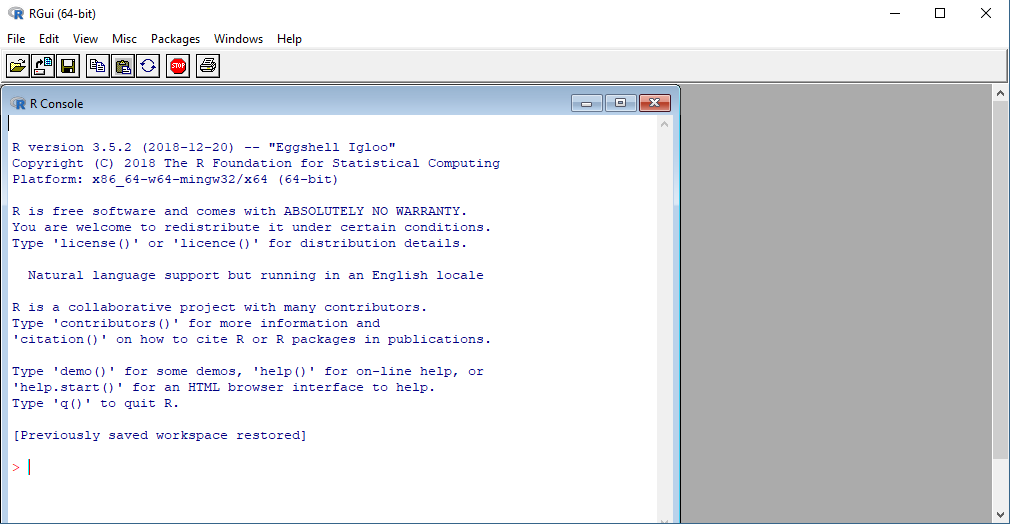
\includegraphics[width=0.8\linewidth]{jendela_r} 

}

\caption{Jendela R.}\label{fig:jendela-R}
\end{figure}

\begin{figure}

{\centering 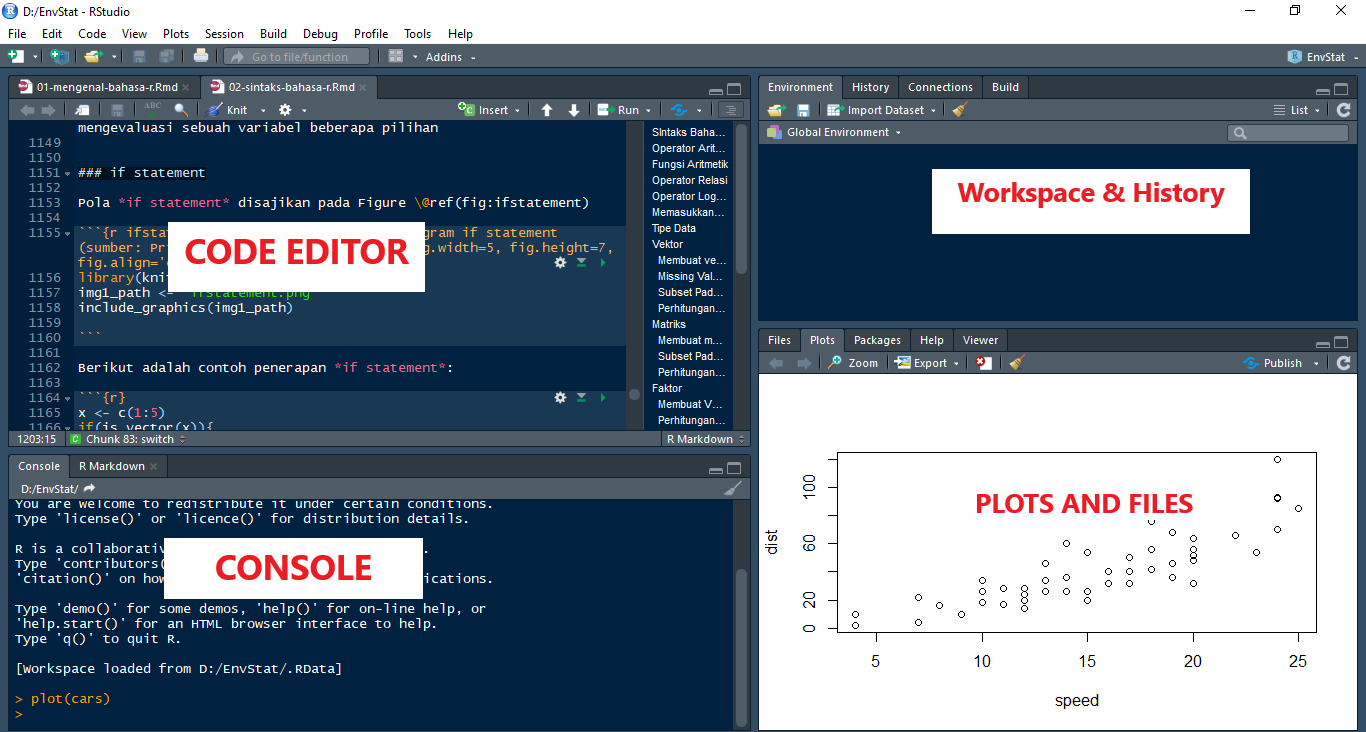
\includegraphics[width=0.8\linewidth]{jendela_rstudio} 

}

\caption{Jendela RStudio.}\label{fig:jendela-RStudio}
\end{figure}

\begin{quote}
\textbf{Note: } Sebaiknya install \texttt{R} terlebih dahulu sebelum
\texttt{RStudio}
\end{quote}

\section{Working Directory}\label{working-directory}

Setiap pengguna akan bekerja pada tempat khusus yang disebut sebagai
\emph{working directory}. \emph{working directory} merupakan sebuah
folder dimana \texttt{R} akan membaca dan menyimpan file kerja kita.
Pada pengguna \texttt{windows}, \emph{working directory} secara default
pada saat pertama kali menginstall \texttt{R} terletak pada folder
\texttt{c:\textbackslash{}\textbackslash{}Document}.

\subsection{Mengubah Lokasi Working
Directory}\label{mengubah-lokasi-working-directory}

Kita dapat mengubah lokasi \emph{working directory} berdasarkan lokasi
yang kita inginkan, misalnya letak data yang akan kita olah tidak ada
pada folder default atau kita ingin pekerjaan kita terkait \texttt{R}
dapat berlangsung pada satu folder khusus.

Berikut adalah cara mengubah \emph{working directory} pada \texttt{R}.

\begin{enumerate}
\def\labelenumi{\arabic{enumi}.}
\tightlist
\item
  Buatlah folder pada drive (kita bisa membuat folder pada selain drive
  c) dan namai dengan nama yang kalian inginkan. Pada tutorial ini
  penulis menggunakan nama folder \texttt{R}.
\item
  Jika pengguna menggunakan \texttt{RStudio}, pada menu \texttt{RStudio}
  pilih \textbf{Session \textgreater{} Set Working Directory
  \textgreater{} Chooses Directory}. Proses tersebut ditampilkan pada
  Figure \ref{fig:working}
\item
  Pilih folder yang telah dibuat pada step 1 sebagai *working directory.
\end{enumerate}

\begin{quote}
\textbf{Note: } Data atau file yang hendak dibaca selama proses kerja
pada \texttt{R} harus selalu diletakkan pada working directory. Jika
tidak maka data atau file tidak akan terbaca.
\end{quote}

Untuk mengecek apakah proses perubahan telah terjadi, kita dapat
mengeceknya dengan menjalankan perintah berikut untuk melihat lokasi
\emph{working directory} kita yang baru.

\begin{Shaded}
\begin{Highlighting}[]
\KeywordTok{getwd}\NormalTok{()}
\end{Highlighting}
\end{Shaded}

\begin{figure}

{\centering 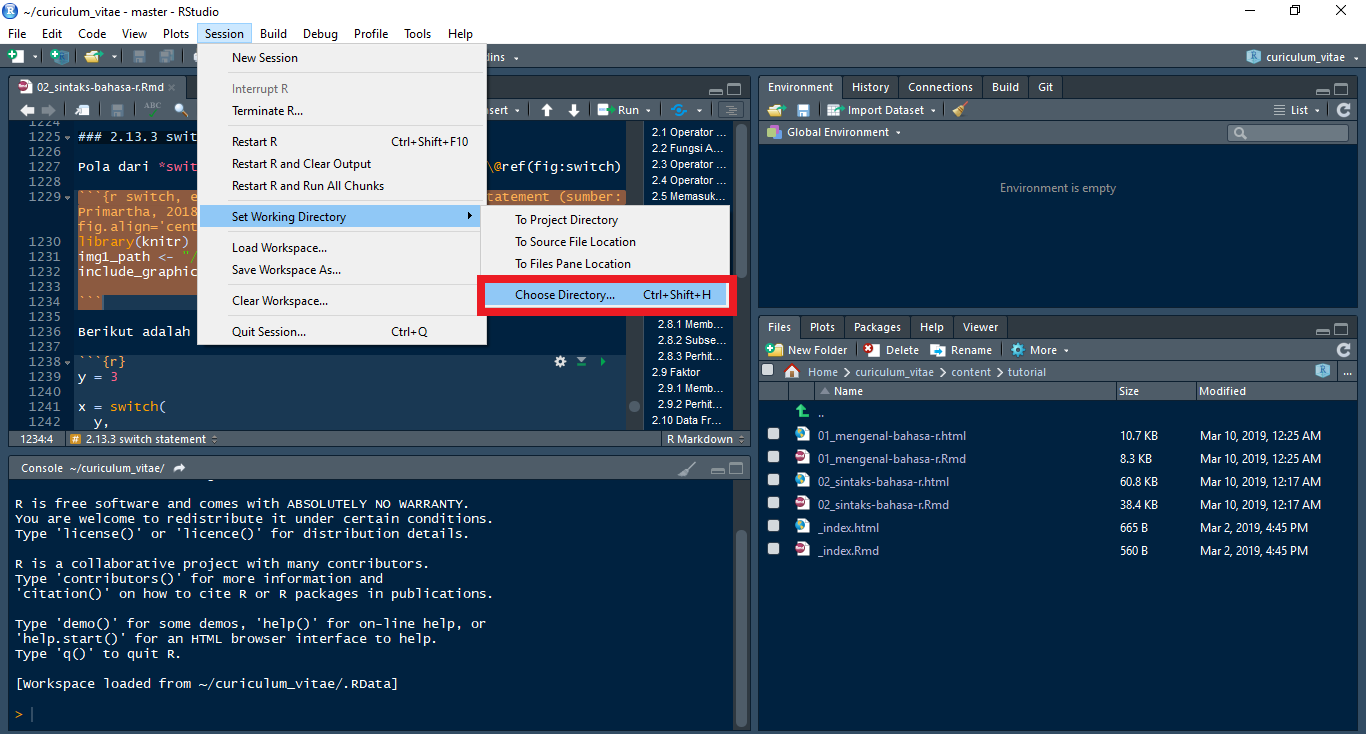
\includegraphics[width=0.8\linewidth]{working} 

}

\caption{Mengubah working directory.}\label{fig:working}
\end{figure}

Selain itu kita dapat mengubah \emph{working directory} menggunakan
perintah berikut:

\begin{Shaded}
\begin{Highlighting}[]
\CommentTok{# Ubah working directori pada folder R}
\KeywordTok{setwd}\NormalTok{(}\StringTok{"/Documents/R"}\NormalTok{)}
\end{Highlighting}
\end{Shaded}

\begin{quote}
\textbf{Note: } Pada proses pengisian lokasi folder pastikan pemisah
pada lokasi folder menggunakan tanda ``/'' bukan ``"
\end{quote}

\subsection{Mengubah Lokasi Working Directory
Default}\label{mengubah-lokasi-working-directory-default}

Pada proses yang telah penulis jelaskan sebelumnya. Proses perubahan
\emph{working directory} hanya berlaku pada saat pekerjaan tersebut
dilakukan. Setelah pekerjaan selesai dan kita menjalankan kembali
\texttt{R} maka \emph{working directory} akan kembali secara default
pada working directory lama.

Untuk membuat lokasi default \emph{working directory} pindah, kita dapat
melakukannya dengan memilih pada menu: \textbf{Tools \textgreater{}
Global options \textgreater{} pada ``General'' klik pada ``Browse'' dan
pilih lokasi working directory yang diinginkan}. Proses tersebut
ditampilkan pada Figure \ref{fig:default}

\begin{figure}

{\centering 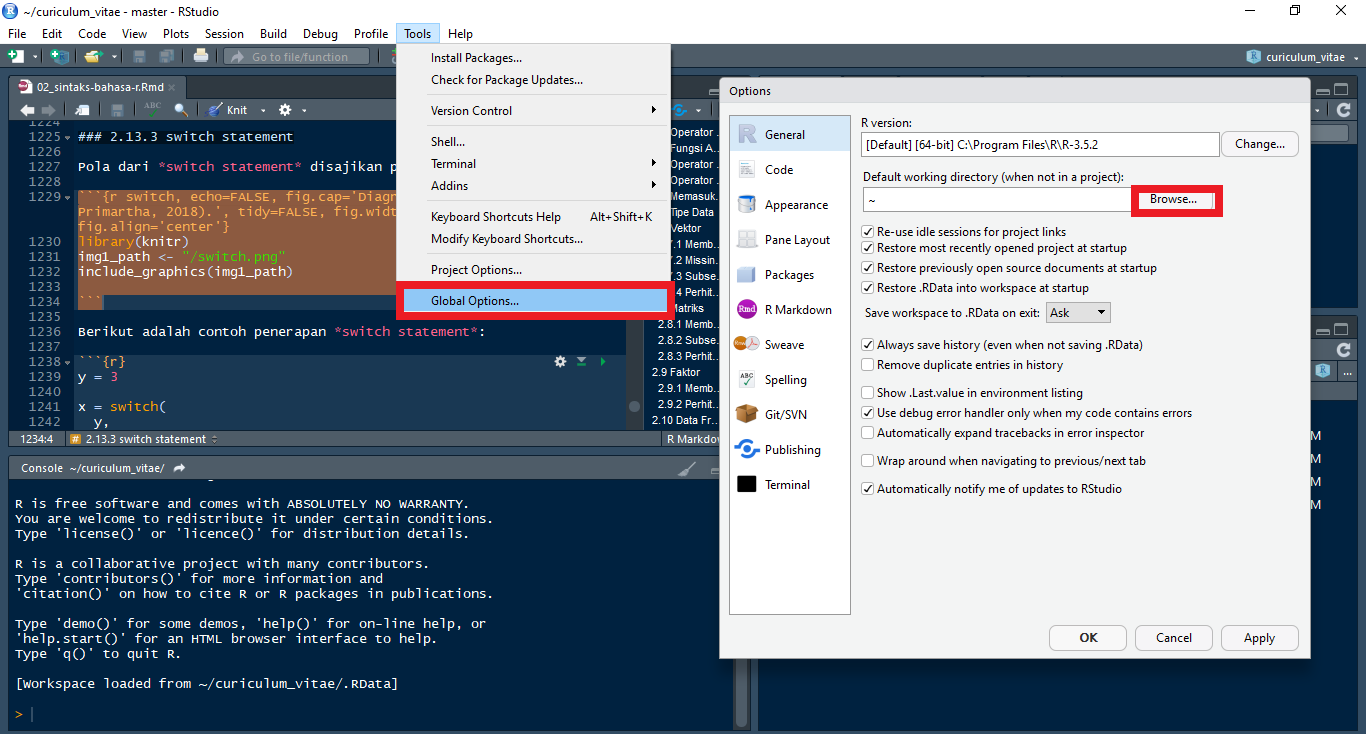
\includegraphics[width=0.8\linewidth]{default} 

}

\caption{Merubah working directory melalui Global options.}\label{fig:default}
\end{figure}

\section{Fasilitas Help}\label{fasilitas-help}

Agar dapat menggunakan \texttt{R} dengan secara lebih baik, pengetahuan
untuk mengakses fasilitas \emph{help} in cukup penting untuk
disampaikan. Adapun cara yang dapat digunakan adalah sebagai berikut.

\subsection{Mencari Help dari Suatu Perintah
Tertentu}\label{mencari-help-dari-suatu-perintah-tertentu}

Untuk memperoleh bantuan terkait suatu perintah tertentu kita dapat
menggunakan fungsi \texttt{help()}. Secara umum format yang digunakan
adalah sebagai berikut:

\begin{Shaded}
\begin{Highlighting}[]
\KeywordTok{help}\NormalTok{(nama_perintah)}
\end{Highlighting}
\end{Shaded}

atau dapat juga menggunakan tanda tanya (?) pada awal
\texttt{nama\_perintah} seperti berikut:

\begin{Shaded}
\begin{Highlighting}[]
\NormalTok{?nama_perintah}
\end{Highlighting}
\end{Shaded}

Misalkan kita kebingungan terkait bagaimana cara menuliskan perintah
untuk menghitung rata-rata suatu vektor. Kita dapat mengetikkan perintah
berikut untuk mengakses fasilitas \emph{help}.

\begin{Shaded}
\begin{Highlighting}[]
\KeywordTok{help}\NormalTok{(mean)}

\CommentTok{#atau}
\NormalTok{?mean}
\end{Highlighting}
\end{Shaded}

Perintah tersebut akan memunculkan hasil berupa dokumentasi yang
ditampilkan pada Figure \ref{fig:meandoc}.

\begin{figure}

{\centering 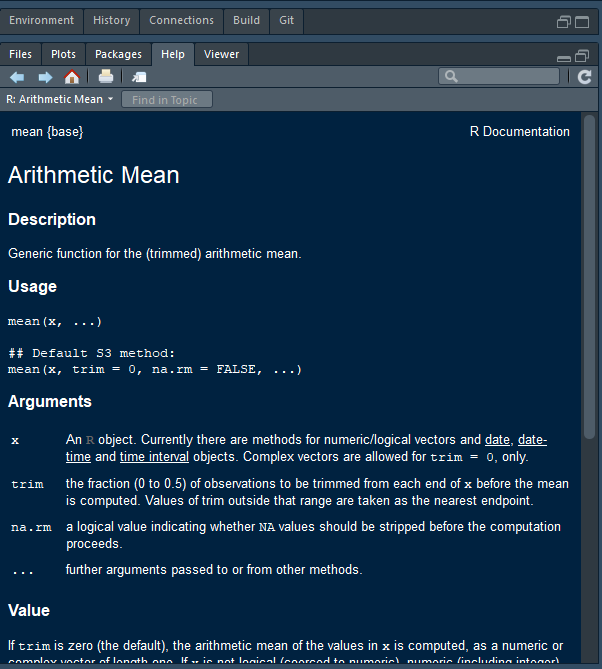
\includegraphics[width=0.5\linewidth]{meandoc} 

}

\caption{Jendela help dokumentasi fungsi mean().}\label{fig:meandoc}
\end{figure}

Keterangan pada jendela pada Figure \ref{fig:meandoc} adalah sebagia
berikut:

\begin{enumerate}
\def\labelenumi{\arabic{enumi}.}
\tightlist
\item
  Pada bagian jendela kiri atas jendela \emph{help}, diberikan
  keterangan nama dari perintah yang sedang ditampilkan.
\item
  Selanjutnya, pada bagian atas dokumen, ditampilkan infomasi terkait
  nama perintah, dan nama \emph{library} yang memuat perintah tersebut.
  Pada gambar diatas informasi terkait perintah dan nama \emph{library}
  ditunjukkan pada teks \texttt{mean\ \{base\}} yang menunjukkan
  perintah \texttt{mean()} pada paket (\emph{library}) \emph{base}
  (paket bawaan \texttt{R}).
\item
  Setiap jendela \emph{help} dari suatu perintah tertentu selanjutnya
  akan memuat bagian-bagian berikut:
\end{enumerate}

\begin{itemize}
\tightlist
\item
  \emph{Title}
\item
  \emph{Description} : deskripsi singkat tentang perintah.
\item
  \emph{Usage} : menampilkan sintaks perintah untuk penggunaan perintah
  tersebut.
\item
  \emph{Arguments} : keterangan mengenai \emph{argument/input}yang
  diperlukan pada perintah tersebut.
\item
  \emph{Details} : keterangan lebih lengkap lengkap tentang perintah
  tersebut.
\item
  \emph{Value} : keterangan tentang \emph{output} suatu perintah dapat
  diperoleh pada bagian ini.
\item
  \emph{Author(s)} : memberikan keterangan tentang \emph{Author} dari
  perintah tersebut.
\item
  \emph{References} : seringkali referensi yang dapat digunakan untuk
  memperoleh keterangan lebih lanjut terhadap suatu perintah ditampilkan
  pada bagian ini.
\item
  \emph{See also}: bagian ini berisikan daftar perintah/fungsi yang
  berhubungan erat dengan perintah tersebut.
\item
  \emph{Example} : berisikan contoh-contoh penggunaan perintah tersebut.
\end{itemize}

Kita juga dapat melihat contoh penggunaan dari perintah tersebut. Untuk
melakukannya kita dapat menggunakan fungsi \texttt{example()}. Fungsi
tersebut akan menampilkan contoh kode penerapan dari fungsi yang kita
inginkan. Secara sederhana fungsi tersebut dapat dituliskan sebagai
berikut:

\begin{Shaded}
\begin{Highlighting}[]
\KeywordTok{example}\NormalTok{(nama_perintah)}
\end{Highlighting}
\end{Shaded}

Untuk mengetahui contoh kode fungsi \texttt{mean()}, ketikkan sintaks
berikut:

\begin{Shaded}
\begin{Highlighting}[]
\KeywordTok{example}\NormalTok{(mean)}
\end{Highlighting}
\end{Shaded}

\begin{verbatim}
## 
## mean> x <- c(0:10, 50)
## 
## mean> xm <- mean(x)
## 
## mean> c(xm, mean(x, trim = 0.10))
## [1] 8.75 5.50
\end{verbatim}

kita juga dapat mencoba kode yang dihasilkan pada console \texttt{R}.
Berikut adalah contoh penerapannya:

\begin{Shaded}
\begin{Highlighting}[]
\CommentTok{# Menghitung rata-rata bilangan 1 sampai 10 dan 50}
\CommentTok{# membuat vektor}
\NormalTok{x <-}\StringTok{ }\KeywordTok{c}\NormalTok{(}\DecValTok{0}\OperatorTok{:}\DecValTok{10}\NormalTok{, }\DecValTok{50}\NormalTok{)}

\CommentTok{# Print}
\NormalTok{x}
\end{Highlighting}
\end{Shaded}

\begin{verbatim}
##  [1]  0  1  2  3  4  5  6  7  8  9 10 50
\end{verbatim}

\begin{Shaded}
\begin{Highlighting}[]
\CommentTok{# mean}
\KeywordTok{mean}\NormalTok{(x)}
\end{Highlighting}
\end{Shaded}

\begin{verbatim}
## [1] 8.75
\end{verbatim}

Pembaca dapat mencoba melakukanya sendiri dengan mengganti nilai yang
telah ada serta mencoba contoh kode yang lain.

\subsection{General Help}\label{general-help}

Kita juga dapat membaca beberapa dokumen manual yang ada pada
\texttt{R}. Untuk melakukannya jalankan perintah berikut:

\begin{Shaded}
\begin{Highlighting}[]
\KeywordTok{help.start}\NormalTok{()}
\end{Highlighting}
\end{Shaded}

Output yang dihasilkan berupa link pada sejumlah dokumen yang dapat kita
klik. Tampilan halaman yang dihasilkan disajikan pada Figure
\ref{fig:generalhelp}.

\begin{figure}

{\centering 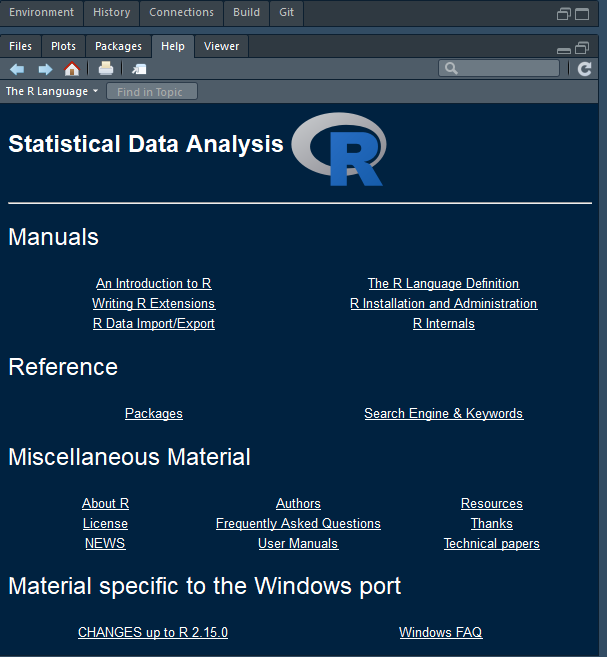
\includegraphics[width=0.5\linewidth]{generalhelp} 

}

\caption{Jendela general help dokumentasi fungsi mean().}\label{fig:generalhelp}
\end{figure}

\subsection{Fasilitas Help Lainnya}\label{fasilitas-help-lainnya}

Selain yang telah penulis sebutkan sebelumnya. Kita juga dapat
memanfaatkan fasilitas \emph{help} lainnya melalui fungsi
\texttt{apropos()} dan \texttt{help.search()}.

\texttt{apropos\ ()}: mengembalikan daftar objek, berisi pola yang
pembaca cari, dengan pencocokan sebagian. Ini berguna ketika pembaca
tidak ingat persis nama fungsi yang akan digunakan. Berikut adalah
contoh ketika penulis ingin mengetahui fungsi yang digunakan untuk
menghitung median.

\begin{Shaded}
\begin{Highlighting}[]
\KeywordTok{apropos}\NormalTok{(}\StringTok{"med"}\NormalTok{)}
\end{Highlighting}
\end{Shaded}

\begin{verbatim}
## [1] "elNamed"        "elNamed<-"      "median"         "median.default"
## [5] "medpolish"      "runmed"
\end{verbatim}

\emph{List} yang dihasilkan berupa fungsi-fungsi yang memiliki elemen
kata ``med''. Berdasarkan pencaria tersebut penulis dapat mencoba
menggunakan fungsi ``median'' untuk menghitung median.

\texttt{help.search\ ()} (sebagai alternatif ??): mencari dokumentasi
yang cocok dengan karakter yang diberikan dengan cara yang berbeda. Ini
mengembalikan daftar fungsi yang mengandung istilah yang pembaca cari
dengan deskripsi singkat dari fungsi.

Berikut adalah contoh penerapan dari fungsi tersebut:

\begin{Shaded}
\begin{Highlighting}[]
\KeywordTok{help.search}\NormalTok{(}\StringTok{"mean"}\NormalTok{)}

\CommentTok{# atau}
\NormalTok{??mean}
\end{Highlighting}
\end{Shaded}

\emph{Output} yang dihasilkan akan tampak seperti pada Figure
\ref{fig:helpsearch}.

\begin{figure}

{\centering 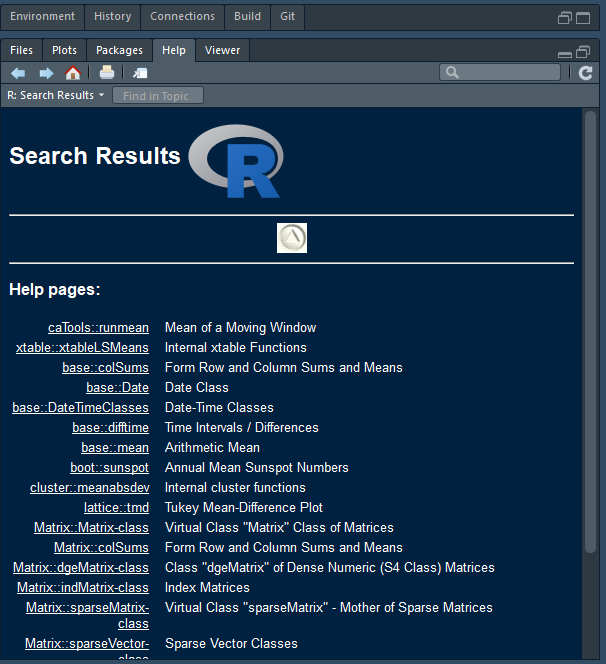
\includegraphics[width=0.5\linewidth]{helpsearch} 

}

\caption{Jendela help search dokumentasi fungsi mean().}\label{fig:helpsearch}
\end{figure}

\section{Referensi}\label{referensi}

\begin{enumerate}
\def\labelenumi{\arabic{enumi}.}
\tightlist
\item
  Primartha, R. 2018. \textbf{Belajar Machine Learning Teori dan
  Praktik}. Penerbit Informatika : Bandung
\item
  Rosadi,D. 2016. \textbf{Analisis Statistika dengan R}. Gadjah Mada
  University Press: Yogyakarta
\item
  STHDA. Running RStudio and Setting Up Your Working Directory - Easy R
  Programming
  .\url{http://www.sthda.com/english/wiki/running-rstudio-and-setting-up-your-working-directory-easy-r-programming\#set-your-working-directory}
\item
  STDHA. \textbf{Getting Help With Functions In R Programming}.
  \url{http://www.sthda.com/english/wiki/getting-help-with-functions-in-r-programming}
  .
\item
  Venables, W.N. Smith D.M. and R Core Team. 2018. \textbf{An
  Introduction to R}. R Manuals.
\end{enumerate}

\chapter{Sintaks Bahasa R}\label{sintaks-bahasa-r}

\section{Operator Aritmatika}\label{operator-aritmatika}

Proses perhitungan akan ditangani oleh fungsi khusus. \texttt{R} akan
memahami urutannya secara benar. Kecuali kita secara eksplisit
menetapkan yang lain. Sebagai contoh jalankan sintaks berikut:

\begin{Shaded}
\begin{Highlighting}[]
\DecValTok{2}\OperatorTok{+}\DecValTok{4}\OperatorTok{*}\DecValTok{2}
\end{Highlighting}
\end{Shaded}

\begin{verbatim}
## [1] 10
\end{verbatim}

Bandingkan dengan sintaks berikut:

\begin{Shaded}
\begin{Highlighting}[]
\NormalTok{(}\DecValTok{2}\OperatorTok{+}\DecValTok{4}\NormalTok{)}\OperatorTok{*}\DecValTok{2}
\end{Highlighting}
\end{Shaded}

\begin{verbatim}
## [1] 12
\end{verbatim}

\begin{quote}
\texttt{R} dapat digunakan sebagai kalkulator
\end{quote}

Berdasarkan kedua hasil tersebut dapat disimpulkan bahwa ketika kita
tidak menetapkan urutan perhitungan menggunakan tanda kurung, \texttt{R}
akan secara otomatis akan menghitung terlebih dahulu perkalian atau
pembangian.

Operator aritmatika yang disediakan \texttt{R} adalah sebagai berikut:

\textbf{Table 1} Operator Aritmatika \texttt{R}

\begin{longtable}[]{@{}ll@{}}
\toprule
\begin{minipage}[b]{0.15\columnwidth}\raggedright\strut
\textbf{Simbol}\strut
\end{minipage} & \begin{minipage}[b]{0.79\columnwidth}\raggedright\strut
\textbf{Keterangan}\strut
\end{minipage}\tabularnewline
\midrule
\endhead
\begin{minipage}[t]{0.15\columnwidth}\raggedright\strut
+\strut
\end{minipage} & \begin{minipage}[t]{0.79\columnwidth}\raggedright\strut
\emph{Addition}, untuk operasi penjumlahan\strut
\end{minipage}\tabularnewline
\begin{minipage}[t]{0.15\columnwidth}\raggedright\strut
-\strut
\end{minipage} & \begin{minipage}[t]{0.79\columnwidth}\raggedright\strut
\emph{Substraction}, untuk operasi pengurangan\strut
\end{minipage}\tabularnewline
\begin{minipage}[t]{0.15\columnwidth}\raggedright\strut
*\strut
\end{minipage} & \begin{minipage}[t]{0.79\columnwidth}\raggedright\strut
\emph{Multiplication}, untuk operasi pembagian\strut
\end{minipage}\tabularnewline
\begin{minipage}[t]{0.15\columnwidth}\raggedright\strut
/\strut
\end{minipage} & \begin{minipage}[t]{0.79\columnwidth}\raggedright\strut
\emph{Division}, untuk operasi pembagian\strut
\end{minipage}\tabularnewline
\begin{minipage}[t]{0.15\columnwidth}\raggedright\strut
\^{}\strut
\end{minipage} & \begin{minipage}[t]{0.79\columnwidth}\raggedright\strut
\emph{Eksponentiation}, untuk operasi pemangkatan\strut
\end{minipage}\tabularnewline
\begin{minipage}[t]{0.15\columnwidth}\raggedright\strut
\%\%\strut
\end{minipage} & \begin{minipage}[t]{0.79\columnwidth}\raggedright\strut
\emph{Modulus}, Untuk mencari sisa pembagian\strut
\end{minipage}\tabularnewline
\begin{minipage}[t]{0.15\columnwidth}\raggedright\strut
\%/\%\strut
\end{minipage} & \begin{minipage}[t]{0.79\columnwidth}\raggedright\strut
\emph{Integer}, Untuk mencari bilangan bulat hasil pembagian saja dan
tanpa sisa pembagian\strut
\end{minipage}\tabularnewline
\bottomrule
\end{longtable}

Untuk lebih memahaminya berikut contoh sintaks penerapan operator
tersebut.

\begin{Shaded}
\begin{Highlighting}[]
\CommentTok{# Addition}
\DecValTok{5}\OperatorTok{+}\DecValTok{3}
\end{Highlighting}
\end{Shaded}

\begin{verbatim}
## [1] 8
\end{verbatim}

\begin{Shaded}
\begin{Highlighting}[]
\CommentTok{# Substraction}
\DecValTok{5}\OperatorTok{-}\DecValTok{3}
\end{Highlighting}
\end{Shaded}

\begin{verbatim}
## [1] 2
\end{verbatim}

\begin{Shaded}
\begin{Highlighting}[]
\CommentTok{# Multiplication}
\DecValTok{5}\OperatorTok{*}\DecValTok{3}
\end{Highlighting}
\end{Shaded}

\begin{verbatim}
## [1] 15
\end{verbatim}

\begin{Shaded}
\begin{Highlighting}[]
\CommentTok{# Division}
\DecValTok{5}\OperatorTok{/}\DecValTok{3}
\end{Highlighting}
\end{Shaded}

\begin{verbatim}
## [1] 1.666667
\end{verbatim}

\begin{Shaded}
\begin{Highlighting}[]
\CommentTok{# Eksponetiation}
\DecValTok{5}\OperatorTok{^}\DecValTok{3}
\end{Highlighting}
\end{Shaded}

\begin{verbatim}
## [1] 125
\end{verbatim}

\begin{Shaded}
\begin{Highlighting}[]
\CommentTok{# Modulus}
\DecValTok{5}\OperatorTok\DecValTok{3}
\end{Highlighting}
\end{Shaded}

\begin{verbatim}
## [1] 2
\end{verbatim}

\begin{Shaded}
\begin{Highlighting}[]
\CommentTok{# Integer}
\DecValTok{5}\OperatorTok\DecValTok{3}
\end{Highlighting}
\end{Shaded}

\begin{verbatim}
## [1] 1
\end{verbatim}

\begin{quote}
\emph{Note: } Pada \texttt{R} tanda \texttt{\#} berfungsi menambahkan
keterangan untuk menjelaskan sebuah sintaks pada \texttt{R}.
\end{quote}

\section{Fungsi Aritmetik}\label{fungsi-aritmetik}

Selain fungsi operator aritmetik, pada \texttt{R} juga telah tersedia
fungsi aritmetik yang lain seperti logaritmik, ekponensial,
trigonometri, dll.

\begin{enumerate}
\def\labelenumi{\arabic{enumi}.}
\tightlist
\item
  Logaritma dan eksponensial
\end{enumerate}

Untuk contoh fungsi logaritmik dan eksponensial jalankan sintaks
berikut:

\begin{Shaded}
\begin{Highlighting}[]
\KeywordTok{log2}\NormalTok{(}\DecValTok{8}\NormalTok{) }\CommentTok{# logaritma basis 2 untuk 8}
\end{Highlighting}
\end{Shaded}

\begin{verbatim}
## [1] 3
\end{verbatim}

\begin{Shaded}
\begin{Highlighting}[]
\KeywordTok{log10}\NormalTok{(}\DecValTok{8}\NormalTok{) }\CommentTok{# logaritma basis 10 untuk 8}
\end{Highlighting}
\end{Shaded}

\begin{verbatim}
## [1] 0.90309
\end{verbatim}

\begin{Shaded}
\begin{Highlighting}[]
\KeywordTok{exp}\NormalTok{(}\DecValTok{8}\NormalTok{) }\CommentTok{# eksponensial 8}
\end{Highlighting}
\end{Shaded}

\begin{verbatim}
## [1] 2980.958
\end{verbatim}

\begin{enumerate}
\def\labelenumi{\arabic{enumi}.}
\setcounter{enumi}{1}
\tightlist
\item
  Fungsi trigonometri
\end{enumerate}

fungsi trigonometri yang ditampilkan seperti sin,cos, tan, dll.

\begin{Shaded}
\begin{Highlighting}[]
\KeywordTok{cos}\NormalTok{(x) }\CommentTok{# cos x}
\KeywordTok{sin}\NormalTok{(x) }\CommentTok{# Sin x}
\KeywordTok{tan}\NormalTok{(x) }\CommentTok{# Tan x}
\KeywordTok{acos}\NormalTok{(x) }\CommentTok{# arc-cos x}
\KeywordTok{asin}\NormalTok{(x) }\CommentTok{# arc-sin x}
\KeywordTok{atan}\NormalTok{(x) }\CommentTok{#arc-tan x}
\end{Highlighting}
\end{Shaded}

\begin{quote}
\textbf{Note: } x dalam fungsi trigonometri memiliki satuan radian
\end{quote}

Berikut adalah salah satu contoh penggunaannya:

\begin{Shaded}
\begin{Highlighting}[]
\KeywordTok{cos}\NormalTok{(pi)}
\end{Highlighting}
\end{Shaded}

\begin{verbatim}
## [1] -1
\end{verbatim}

\begin{enumerate}
\def\labelenumi{\arabic{enumi}.}
\setcounter{enumi}{2}
\tightlist
\item
  Fungsi matematik lainnya
\end{enumerate}

Fungsi lainnya yang dapat digunakan adalah fungsi absolut, akar kuadrat,
dll. Berikut adalah contoh sintaks penggunaan fungsi absolut dan akar
kuadrat.

\begin{Shaded}
\begin{Highlighting}[]
\KeywordTok{abs}\NormalTok{(}\OperatorTok{-}\DecValTok{2}\NormalTok{) }\CommentTok{# nilai absolut -2}
\end{Highlighting}
\end{Shaded}

\begin{verbatim}
## [1] 2
\end{verbatim}

\begin{Shaded}
\begin{Highlighting}[]
\KeywordTok{sqrt}\NormalTok{(}\DecValTok{4}\NormalTok{) }\CommentTok{# akar kuadrat 4}
\end{Highlighting}
\end{Shaded}

\begin{verbatim}
## [1] 2
\end{verbatim}

\section{Operator Relasi}\label{operator-relasi}

Operator relasi digunakan untuk membandingkan satu objek dengan objek
lainnya. Operator yang disediakan \texttt{R} disajikan pada Table 2.

\textbf{Table 2} Operator Relasi \texttt{R}

\begin{longtable}[]{@{}ll@{}}
\toprule
\textbf{Simbol} & \textbf{Keterangan}\tabularnewline
\midrule
\endhead
``\textgreater{}'' & Lebih besar dari\tabularnewline
``\textless{}'' & Lebih Kecil dari\tabularnewline
``=='' & Sama dengan\tabularnewline
``\textgreater{}='' & Lebih besar sama dengan\tabularnewline
``\textless{}='' & Lebih kecil sama dengan\tabularnewline
``!='' & Tidak sama dengan\tabularnewline
\bottomrule
\end{longtable}

Berikut adalah penerapan operator pada tabel tersebut:

\begin{Shaded}
\begin{Highlighting}[]
\NormalTok{x <-}\StringTok{ }\DecValTok{34}
\NormalTok{y <-}\StringTok{ }\DecValTok{35}

\CommentTok{# Operator >}
\NormalTok{x }\OperatorTok{>}\StringTok{ }\NormalTok{y}
\end{Highlighting}
\end{Shaded}

\begin{verbatim}
## [1] FALSE
\end{verbatim}

\begin{Shaded}
\begin{Highlighting}[]
\CommentTok{# Operator <}
\NormalTok{x }\OperatorTok{<}\StringTok{ }\NormalTok{y}
\end{Highlighting}
\end{Shaded}

\begin{verbatim}
## [1] TRUE
\end{verbatim}

\begin{Shaded}
\begin{Highlighting}[]
\CommentTok{# operator ==}
\NormalTok{x }\OperatorTok{==}\StringTok{ }\NormalTok{y}
\end{Highlighting}
\end{Shaded}

\begin{verbatim}
## [1] FALSE
\end{verbatim}

\begin{Shaded}
\begin{Highlighting}[]
\CommentTok{# Operator >=}
\NormalTok{x }\OperatorTok{>=}\StringTok{ }\NormalTok{y}
\end{Highlighting}
\end{Shaded}

\begin{verbatim}
## [1] FALSE
\end{verbatim}

\begin{Shaded}
\begin{Highlighting}[]
\CommentTok{# Operator <=}
\NormalTok{x }\OperatorTok{<=}\StringTok{ }\NormalTok{y}
\end{Highlighting}
\end{Shaded}

\begin{verbatim}
## [1] TRUE
\end{verbatim}

\begin{Shaded}
\begin{Highlighting}[]
\CommentTok{# Operator !=}
\NormalTok{x }\OperatorTok{!=}\StringTok{ }\NormalTok{y}
\end{Highlighting}
\end{Shaded}

\begin{verbatim}
## [1] TRUE
\end{verbatim}

\section{Operator Logika}\label{operator-logika}

Operator logika hanya berlaku pada vektor dengan tipe logical, numeric,
atau complex. Semua angka bernilai 1 akan dianggap bernilai logika
\texttt{TRUE}. Operator logika yang disediakan \texttt{R} dapat dilihat
pada Table 3.

\textbf{Table 3} Operator logika \texttt{R}

\begin{longtable}[]{@{}ll@{}}
\toprule
\textbf{Simbol} & \textbf{Keterangan}\tabularnewline
\midrule
\endhead
\&\& & Operator logika AND\tabularnewline
&\tabularnewline
! & Opeartor logika NOT\tabularnewline
\& & Operator logika AND element wise\tabularnewline
& Operator logika OR element wise\tabularnewline
\bottomrule
\end{longtable}

Penerapannya terdapat pada sintaks berikut:

\begin{Shaded}
\begin{Highlighting}[]
\NormalTok{v <-}\StringTok{ }\KeywordTok{c}\NormalTok{(}\OtherTok{TRUE}\NormalTok{,}\OtherTok{TRUE}\NormalTok{, }\OtherTok{FALSE}\NormalTok{)}
\NormalTok{t <-}\StringTok{ }\KeywordTok{c}\NormalTok{(}\OtherTok{FALSE}\NormalTok{,}\OtherTok{FALSE}\NormalTok{,}\OtherTok{FALSE}\NormalTok{)}

\CommentTok{# Operator &&}
\KeywordTok{print}\NormalTok{(v}\OperatorTok{&&}\NormalTok{t)}
\end{Highlighting}
\end{Shaded}

\begin{verbatim}
## [1] FALSE
\end{verbatim}

\begin{Shaded}
\begin{Highlighting}[]
\CommentTok{# Operator ||}
\KeywordTok{print}\NormalTok{(v}\OperatorTok{||}\NormalTok{t)}
\end{Highlighting}
\end{Shaded}

\begin{verbatim}
## [1] TRUE
\end{verbatim}

\begin{Shaded}
\begin{Highlighting}[]
\CommentTok{# Operator !}
\KeywordTok{print}\NormalTok{(}\OperatorTok{!}\NormalTok{v)}
\end{Highlighting}
\end{Shaded}

\begin{verbatim}
## [1] FALSE FALSE  TRUE
\end{verbatim}

\begin{Shaded}
\begin{Highlighting}[]
\CommentTok{# operator &}
\KeywordTok{print}\NormalTok{(v}\OperatorTok{&}\NormalTok{t)}
\end{Highlighting}
\end{Shaded}

\begin{verbatim}
## [1] FALSE FALSE FALSE
\end{verbatim}

\begin{Shaded}
\begin{Highlighting}[]
\CommentTok{# Operator |}
\KeywordTok{print}\NormalTok{(v}\OperatorTok{|}\NormalTok{t)}
\end{Highlighting}
\end{Shaded}

\begin{verbatim}
## [1]  TRUE  TRUE FALSE
\end{verbatim}

\begin{quote}
\textbf{Note: }

operator \& dan \textbar{} akan mengecek logika tiap elemen pada vektor
secara berpesangan (sesuai urutan dari kiri ke kanan).

Operator \%\% dan \textbar{}\textbar{} hanya mengecek dari kiri ke kanan
pada observasi pertama. Misal saat menggunakan \&\& jika observasi
pertama TRUE maka observasi pertama pada vektor lainnya akan dicek,
namun jika observasi pertama FALSE maka proses akan segera dihentikan
dan menghasilkan FALSE.
\end{quote}

\section{Memasukkan Nilai Kedalam
Variabel}\label{memasukkan-nilai-kedalam-variabel}

Variabel pada \texttt{R} dapat digunakan untuk menyimpan nilai. Sebagai
contoh jalankan sintaks berikut:

\begin{Shaded}
\begin{Highlighting}[]
\CommentTok{# Harga sebuah lemon adalah 500 rupiah}
\NormalTok{lemon <-}\StringTok{ }\DecValTok{500}

\CommentTok{# Atau}
\DecValTok{500}\NormalTok{ ->}\StringTok{ }\NormalTok{lemon}

\CommentTok{# dapat juga menggunakan tanda "="}
\NormalTok{lemon =}\StringTok{ }\DecValTok{500}
\end{Highlighting}
\end{Shaded}

\begin{quote}
\textbf{Note: }

\begin{enumerate}
\def\labelenumi{\arabic{enumi}.}
\item
  \texttt{R} memungkinkan penggunaan \textless{}-,-\textgreater{}, atau
  = sebagai perintah pengisi nilai variabel
\item
  \texttt{R} bersifat \emph{case-sensitive}. Maksudnya adalah variabel
  Lemon tidak sama dengan lemon (Besar kecil huruf berpengaruh)
\end{enumerate}
\end{quote}

Untuk mengetahui nilai dari objek \texttt{lemon} kita dapat menggunakan
fungsi \texttt{print()} atau mengetikkan nama objeknya secara langsung.

\begin{Shaded}
\begin{Highlighting}[]
\CommentTok{# Menggunakan fungsi print()}
\KeywordTok{print}\NormalTok{(lemon)}
\end{Highlighting}
\end{Shaded}

\begin{verbatim}
## [1] 500
\end{verbatim}

\begin{Shaded}
\begin{Highlighting}[]
\CommentTok{# Atau}
\NormalTok{lemon}
\end{Highlighting}
\end{Shaded}

\begin{verbatim}
## [1] 500
\end{verbatim}

\texttt{R} akan menyimpan variabel \texttt{lemon} sebagai objek pada
memori. Sehingga kita dapat melakukan operasi terhadap objek tersebut
seperti mengalikannya atau menjumlahkannya dengan bilangan lain. Sebagai
contoh jalankan sintaks berikut:

\begin{Shaded}
\begin{Highlighting}[]
\CommentTok{# Operasi perkalian terhadap objek lemon}
\DecValTok{5}\OperatorTok{*}\NormalTok{lemon}
\end{Highlighting}
\end{Shaded}

\begin{verbatim}
## [1] 2500
\end{verbatim}

Kita dapat juga mengubah nilai dari objek \texttt{lemon} dengan cara
menginput nilai baru terhadap objek yang sama. \texttt{R} secara
otomatis akan menggatikan nilai sebelumnya. Untuk lebih memahaminya
jalankan sintaks berikut:

\begin{Shaded}
\begin{Highlighting}[]
\NormalTok{lemon <-}\StringTok{ }\DecValTok{1000}

\CommentTok{# Print lemon}
\KeywordTok{print}\NormalTok{(lemon)}
\end{Highlighting}
\end{Shaded}

\begin{verbatim}
## [1] 1000
\end{verbatim}

Untuk lebih memahaminya berikut adalah sintaks untuk menghitung volume
suatu objek.

\begin{Shaded}
\begin{Highlighting}[]
\CommentTok{# Dimensi objek}
\NormalTok{panjang <-}\StringTok{ }\DecValTok{10}
\NormalTok{lebar <-}\StringTok{ }\DecValTok{5}
\NormalTok{tinggi <-}\StringTok{ }\DecValTok{5}

\CommentTok{# Menghitung volume}
\NormalTok{volume <-}\StringTok{ }\NormalTok{panjang}\OperatorTok{*}\NormalTok{lebar}\OperatorTok{*}\NormalTok{tinggi}

\CommentTok{# Print objek volume}
\KeywordTok{print}\NormalTok{(volume)}
\end{Highlighting}
\end{Shaded}

\begin{verbatim}
## [1] 250
\end{verbatim}

Untuk mengetahui objek apa saja yang telah kita buat sepanjang artikel
ini kita dapang menggunakan fungsi \texttt{ls()}.

\begin{Shaded}
\begin{Highlighting}[]
\KeywordTok{ls}\NormalTok{()}
\end{Highlighting}
\end{Shaded}

\begin{verbatim}
##  [1] "A"         "B"         "img1_path" "lebar"     "lemon"    
##  [6] "panjang"   "t"         "tinggi"    "v"         "volume"   
## [11] "x"         "xm"        "y"
\end{verbatim}

\begin{quote}
Kumpulan objek yang telah tersimpan dalam memori disebut sebagai
\textbf{workspace}
\end{quote}

Untuk menghapus objek pada memori kita dapat menggunakan fungsi
\texttt{rm()}. Pada sintaks berikut penulis hendak menghapus objek
\texttt{lemon} dan \texttt{volume}.

\begin{Shaded}
\begin{Highlighting}[]
\CommentTok{# Menghapus objek lemon dan volume}
\KeywordTok{rm}\NormalTok{(lemon, volume)}

\CommentTok{# Tampilkan kembali objek yang tersisa}
\KeywordTok{ls}\NormalTok{()}
\end{Highlighting}
\end{Shaded}

\begin{verbatim}
##  [1] "A"         "B"         "img1_path" "lebar"     "panjang"  
##  [6] "t"         "tinggi"    "v"         "x"         "xm"       
## [11] "y"
\end{verbatim}

\begin{quote}
\textbf{Note: } Setiap variabel atau objek yang dibuat akan menempati
sejumlah memori pada komputer sehingga jika kita bekerja dengan jumlah
data yang banyak pastikan kita menghapus seluruh objek pada memori
sebelum memulai kerja.
\end{quote}

\section{Tipe Data}\label{tipe-data}

Data pada \texttt{R} dapat dikelompokan berdasarkan beberapa tipe. Tipe
data pada \texttt{R} disajikan pada Table 4.

\textbf{Table 4} Tipe Data \texttt{R}

\begin{longtable}[]{@{}lll@{}}
\toprule
\textbf{Tipe Data} & \textbf{Contoh} &
\textbf{Keterangan}\tabularnewline
\midrule
\endhead
Logical & TRUE, FALSE & Nilai Boolean\tabularnewline
Numeric & 12.3, 5, 999 & Segala jenis angka\tabularnewline
Integer & 23L, 97L, 3L & Bilangan integer (bilangan
bulat)\tabularnewline
Complex & 2i, 3i, 9i & Bilangan kompleks\tabularnewline
Character & `a', ``b'', ``123'' & Karakter dan string\tabularnewline
Raw & Identik dengan ``hello'' & Segala jenis data yang disimpan sebagai
raw bytes\tabularnewline
\bottomrule
\end{longtable}

Sintaks berikut adalah contoh dari tipe data pada \texttt{R}. Untuk
mengetahui tipa data suatu objek kita dapat menggunakan perintah
\texttt{class()}

\begin{Shaded}
\begin{Highlighting}[]
\CommentTok{# Logical}
\NormalTok{apel <-}\StringTok{ }\OtherTok{TRUE}
\KeywordTok{class}\NormalTok{(apel)}
\end{Highlighting}
\end{Shaded}

\begin{verbatim}
## [1] "logical"
\end{verbatim}

\begin{Shaded}
\begin{Highlighting}[]
\CommentTok{# Numeric}
\NormalTok{x <-}\StringTok{ }\FloatTok{2.3}
\KeywordTok{class}\NormalTok{(x)}
\end{Highlighting}
\end{Shaded}

\begin{verbatim}
## [1] "numeric"
\end{verbatim}

\begin{Shaded}
\begin{Highlighting}[]
\CommentTok{# Integer}
\NormalTok{y <-}\StringTok{ }\NormalTok{2L}
\KeywordTok{class}\NormalTok{(y)}
\end{Highlighting}
\end{Shaded}

\begin{verbatim}
## [1] "integer"
\end{verbatim}

\begin{Shaded}
\begin{Highlighting}[]
\CommentTok{# Compleks}
\NormalTok{z <-}\StringTok{ }\DecValTok{5}\OperatorTok{+}\NormalTok{2i}
\KeywordTok{class}\NormalTok{(z)}
\end{Highlighting}
\end{Shaded}

\begin{verbatim}
## [1] "complex"
\end{verbatim}

\begin{Shaded}
\begin{Highlighting}[]
\CommentTok{# string}
\NormalTok{w <-}\StringTok{ "saya"}
\KeywordTok{class}\NormalTok{(w)}
\end{Highlighting}
\end{Shaded}

\begin{verbatim}
## [1] "character"
\end{verbatim}

\begin{Shaded}
\begin{Highlighting}[]
\CommentTok{# Raw}
\NormalTok{xy <-}\StringTok{ }\KeywordTok{charToRaw}\NormalTok{(}\StringTok{"hello world"}\NormalTok{)}
\KeywordTok{class}\NormalTok{(xy)}
\end{Highlighting}
\end{Shaded}

\begin{verbatim}
## [1] "raw"
\end{verbatim}

Keenam jenis data tersebut disebut sebagai tipe data atomik. Hal ini
disebabkan karena hanya dapat menangani satu tipe data saja. Misalnya
hanya numeric atau hanya integer.

Selain menggunakan fungsi \texttt{class()}, kita dapat pula menggunakan
fungsi \texttt{is\_numeric()}, \texttt{is.character()},
\texttt{is.logical()}, dan sebagainya berdasarkan jenis data apa yang
ingin kita cek. Berbeda dengan fungsi \texttt{class()}, ouput yang
dihasilkan pada fungsi seperti \texttt{is\_numeric()} adalah nilai
Boolean sehingga fungsi ini hanya digunakan untuk mengecek apakah jenis
data pada objek sama seperti yang kita pikirkan. Sebagai contoh
disajikan pada sintaks berikut:

\begin{Shaded}
\begin{Highlighting}[]
\NormalTok{data <-}\StringTok{ }\DecValTok{25}

\CommentTok{# Cek apakah objek berisi data numerik}
\KeywordTok{is.numeric}\NormalTok{(data)}
\end{Highlighting}
\end{Shaded}

\begin{verbatim}
## [1] TRUE
\end{verbatim}

\begin{Shaded}
\begin{Highlighting}[]
\CommentTok{# Cek apakah objek adalah karakter}
\KeywordTok{is.character}\NormalTok{(data)}
\end{Highlighting}
\end{Shaded}

\begin{verbatim}
## [1] FALSE
\end{verbatim}

Kita juga dapat mengubah jenis data menjadi jenis lainnya seperti
integer menjadi numerik atau sebaliknya. Fungsi yang digunakan adalah
\texttt{as.numeric()} jika ingin mengubah suatu jenis data menjadi
numerik. Fungsi lainnya juga dapat digunakan sesuai dengan kita ingin
mengubah jenis data objek menjadi jenis data lainnya.

\begin{Shaded}
\begin{Highlighting}[]
\CommentTok{# Integer}
\NormalTok{apel <-}\StringTok{ }\NormalTok{2L}

\CommentTok{# Ubah menjadi numerik}
\KeywordTok{as.numeric}\NormalTok{(apel)}
\end{Highlighting}
\end{Shaded}

\begin{verbatim}
## [1] 2
\end{verbatim}

\begin{Shaded}
\begin{Highlighting}[]
\CommentTok{# Cek}
\KeywordTok{is.numeric}\NormalTok{(apel)}
\end{Highlighting}
\end{Shaded}

\begin{verbatim}
## [1] TRUE
\end{verbatim}

\begin{Shaded}
\begin{Highlighting}[]
\CommentTok{# Logical}
\NormalTok{nangka <-}\StringTok{ }\OtherTok{TRUE}

\CommentTok{# Ubah logical menjadi numeric}
\KeywordTok{as.numeric}\NormalTok{(nangka)}
\end{Highlighting}
\end{Shaded}

\begin{verbatim}
## [1] 1
\end{verbatim}

\begin{Shaded}
\begin{Highlighting}[]
\CommentTok{# Karakter}
\NormalTok{minum <-}\StringTok{ "minum"}

\CommentTok{# ubah karakter menjadi numerik}
\KeywordTok{as.numeric}\NormalTok{(minum)}
\end{Highlighting}
\end{Shaded}

\begin{verbatim}
## Warning: NAs introduced by coercion
\end{verbatim}

\begin{verbatim}
## [1] NA
\end{verbatim}

\begin{quote}
\textbf{Note: } Konversi karakter menjadi numerik akan menghasilkan
output NA (\emph{not available}). \texttt{R} tidak mengetahui bagaimana
cara merubah karakter menjadi bentuk numerik.
\end{quote}

Berdasarkan Tabel 2, vektor karakter dapat dibuat menggunakan tanda
kurung baik \emph{double quote} (``'') maupun \emph{single quote}
('').Jika pada teks yang kita tuliskan mengandung \emph{quote} maka kita
harus menghentikannya menggunakan tanda ( ~). Sbegai contoh kita ingin
menuliskan `\textbf{My friend's name is ``Adi''}, pada sintaks akan
dituliskan:

\begin{Shaded}
\begin{Highlighting}[]
\StringTok{'My friend\textbackslash{}`s name is "Adi"'}
\end{Highlighting}
\end{Shaded}

\begin{verbatim}
## [1] "My friend`s name is \"Adi\""
\end{verbatim}

\begin{Shaded}
\begin{Highlighting}[]
\CommentTok{# Atau}

\StringTok{"My friend's name }\CharTok{\textbackslash{}"}\StringTok{Adi}\CharTok{\textbackslash{}"}\StringTok{"}
\end{Highlighting}
\end{Shaded}

\begin{verbatim}
## [1] "My friend's name \"Adi\""
\end{verbatim}

\section{Vektor}\label{vektor}

Vektor merupakan kombinasi berbagai nilai (numerik, karakter, logical,
dan sebagainya berdasarkan jenis input data) pada objek yang sma. Pada
contoh kasus berikut, pembaca akan memiliki sesuai jenis data input
yaitu\textbf{vektor numerik}, \textbf{vector karakter}, \textbf{vektor
logical}, dll.

\subsection{Membuat vektor}\label{membuat-vektor}

Vektor dibuat dengan menggunakan fungsi \texttt{c()}(concatenate)
seperti yang disajikan pada sintaks berikut:

\begin{Shaded}
\begin{Highlighting}[]
\CommentTok{# membuat vektor numerik}
\NormalTok{x <-}\StringTok{ }\KeywordTok{c}\NormalTok{(}\DecValTok{3}\NormalTok{,}\FloatTok{3.5}\NormalTok{,}\DecValTok{4}\NormalTok{,}\DecValTok{7}\NormalTok{)}
\NormalTok{x }\CommentTok{# print vektor}
\end{Highlighting}
\end{Shaded}

\begin{verbatim}
## [1] 3.0 3.5 4.0 7.0
\end{verbatim}

\begin{Shaded}
\begin{Highlighting}[]
\CommentTok{# membuat vektor karakter}
\NormalTok{y <-}\StringTok{ }\KeywordTok{c}\NormalTok{(}\StringTok{"Apel"}\NormalTok{, }\StringTok{"Jeruk"}\NormalTok{, }\StringTok{"Rambutan"}\NormalTok{, }\StringTok{"Salak"}\NormalTok{)}
\NormalTok{y }\CommentTok{# print vektor}
\end{Highlighting}
\end{Shaded}

\begin{verbatim}
## [1] "Apel"     "Jeruk"    "Rambutan" "Salak"
\end{verbatim}

\begin{Shaded}
\begin{Highlighting}[]
\CommentTok{# membuat vektor logical}
\NormalTok{t <-}\StringTok{ }\KeywordTok{c}\NormalTok{(}\StringTok{"TRUE"}\NormalTok{, }\StringTok{"FALSE"}\NormalTok{, }\StringTok{"TRUE"}\NormalTok{)}
\NormalTok{t }\CommentTok{# print vektor}
\end{Highlighting}
\end{Shaded}

\begin{verbatim}
## [1] "TRUE"  "FALSE" "TRUE"
\end{verbatim}

selain menginput nilai pada vektor, kita juga dapat memberi nama nilai
setiap vektor menggunakan fungsi \texttt{names()}.

\begin{Shaded}
\begin{Highlighting}[]
\CommentTok{# Membuat vektor jumlah buah yang dibeli}
\NormalTok{Jumlah <-}\StringTok{ }\KeywordTok{c}\NormalTok{(}\DecValTok{5}\NormalTok{,}\DecValTok{5}\NormalTok{,}\DecValTok{6}\NormalTok{,}\DecValTok{7}\NormalTok{)}
\KeywordTok{names}\NormalTok{(Jumlah) <-}\StringTok{ }\KeywordTok{c}\NormalTok{(}\StringTok{"Apel"}\NormalTok{, }\StringTok{"Jeruk"}\NormalTok{, }\StringTok{"Rambutan"}\NormalTok{, }\StringTok{"Salak"}\NormalTok{)}

\CommentTok{# Atau}
\NormalTok{Jumlah <-}\StringTok{ }\KeywordTok{c}\NormalTok{(}\DataTypeTok{Apel=}\DecValTok{5}\NormalTok{, }\DataTypeTok{Jeruk=}\DecValTok{5}\NormalTok{, }\DataTypeTok{Rambutan=}\DecValTok{6}\NormalTok{, }\DataTypeTok{Salak=}\DecValTok{7}\NormalTok{)}

\CommentTok{# Print}
\NormalTok{Jumlah}
\end{Highlighting}
\end{Shaded}

\begin{verbatim}
##     Apel    Jeruk Rambutan    Salak 
##        5        5        6        7
\end{verbatim}

\begin{quote}
\textbf{Note: } Vektor hanya dapat memuat satu buah jenis data. Vektor
hanya dapat mengandung jenis data numerik saja, karakter saja, dll.
\end{quote}

Untuk menentukan panjang sebuah vektor kita dapat menggunakan fungsi
\texttt{lenght()}.

\begin{Shaded}
\begin{Highlighting}[]
\KeywordTok{length}\NormalTok{(Jumlah)}
\end{Highlighting}
\end{Shaded}

\begin{verbatim}
## [1] 4
\end{verbatim}

\subsection{Missing Values}\label{missing-values}

Seringkali nilai pada vektor kita tidak lengkap atau terdapat nilai yang
hilang (\emph{missing value}) pada vektor. \emph{Missing value} pada
\texttt{R} dilambangkan oleh \texttt{NA}(\emph{not available}). Berikut
adalah contoh vektor dengan \emph{missing value}.

\begin{Shaded}
\begin{Highlighting}[]
\NormalTok{Jumlah <-}\StringTok{ }\KeywordTok{c}\NormalTok{(}\DataTypeTok{Apel=}\DecValTok{5}\NormalTok{, }\DataTypeTok{Jeruk=}\OtherTok{NA}\NormalTok{, }\DataTypeTok{Rambutan=}\DecValTok{6}\NormalTok{, }\DataTypeTok{Salak=}\DecValTok{7}\NormalTok{)}
\end{Highlighting}
\end{Shaded}

Untuk mengecek apakah dalam objek terdapat \emph{missing value} dapat
menggunakan fungsi \texttt{is.na()}. ouput dari fungsi tersebut adalah
nilai Boolean. Jika terdapat \emph{Missing value}, maka output yang
dihasilkan akan memberikan nilai \texttt{TRUE}.

\begin{Shaded}
\begin{Highlighting}[]
\KeywordTok{is.na}\NormalTok{(Jumlah)}
\end{Highlighting}
\end{Shaded}

\begin{verbatim}
##     Apel    Jeruk Rambutan    Salak 
##    FALSE     TRUE    FALSE    FALSE
\end{verbatim}

\begin{quote}
\textbf{Note: }

Selain NA terdapat NaN (\emph{not a number}) sebagai \emph{missing
value8}. Nilai tersebut muncul ketika fungsi matematika yang digunakan
pada proses perhitungan tidak bekerja sebagaimana mestinya. Contoh: 0/0
= NaN

\texttt{is.na()} juga akan menghasilkan nilai \texttt{TRUE} pada NaN.
Untuk membedakannya dengan NA dapat digunakan fungsi \texttt{is.nan()}.
\end{quote}

\subsection{Subset Pada Vektor}\label{subset-pada-vektor}

\emph{Subseting vector} terdiri atas tiga jenis, yaitu: \emph{positive
indexing}, \emph{Negative Indexing}, dan .

\begin{itemize}
\tightlist
\item
  \textbf{Positive indexing}: memilih elemen vektor berdasarkan
  posisinya (indeks) dalam kurung siku.
\end{itemize}

\begin{Shaded}
\begin{Highlighting}[]
\CommentTok{# Subset vektor pada urutan kedua}
\NormalTok{Jumlah[}\DecValTok{2}\NormalTok{]}
\end{Highlighting}
\end{Shaded}

\begin{verbatim}
## Jeruk 
##    NA
\end{verbatim}

\begin{Shaded}
\begin{Highlighting}[]
\CommentTok{# Subset vektor pada urutan 2 dan 4}
\NormalTok{Jumlah[}\KeywordTok{c}\NormalTok{(}\DecValTok{2}\NormalTok{, }\DecValTok{4}\NormalTok{)]}
\end{Highlighting}
\end{Shaded}

\begin{verbatim}
## Jeruk Salak 
##    NA     7
\end{verbatim}

Selain melalui urutan (indeks), kita juga dapat melakukan subset
berdasarkan nama elemen vektornya.

\begin{Shaded}
\begin{Highlighting}[]
\NormalTok{Jumlah[}\StringTok{"Jeruk"}\NormalTok{]}
\end{Highlighting}
\end{Shaded}

\begin{verbatim}
## Jeruk 
##    NA
\end{verbatim}

\begin{quote}
\textbf{Note: } Indeks pada \texttt{R} dimulai dari 1. Sehingga kolom
atau elemen pertama vektor dimulai dari {[}1{]}
\end{quote}

\begin{itemize}
\tightlist
\item
  \textbf{Negative indexing}: mengecualikan (\emph{exclude}) elemen
  vektor.
\end{itemize}

\begin{Shaded}
\begin{Highlighting}[]
\CommentTok{# mengecualikan elemen vektor 2 dan 4}
\NormalTok{Jumlah[}\OperatorTok{-}\KeywordTok{c}\NormalTok{(}\DecValTok{2}\NormalTok{,}\DecValTok{4}\NormalTok{)]}
\end{Highlighting}
\end{Shaded}

\begin{verbatim}
##     Apel Rambutan 
##        5        6
\end{verbatim}

\begin{Shaded}
\begin{Highlighting}[]
\CommentTok{# mengecualikan elemen vektor 1 sampai 3}
\NormalTok{Jumlah[}\OperatorTok{-}\KeywordTok{c}\NormalTok{(}\DecValTok{1}\OperatorTok{:}\DecValTok{3}\NormalTok{)]}
\end{Highlighting}
\end{Shaded}

\begin{verbatim}
## Salak 
##     7
\end{verbatim}

\begin{itemize}
\tightlist
\item
  \textbf{Subset berdasarkan vektor logical}: Hanya, elemen-elemen yang
  nilai yang bersesuaian dalam vektor pemilihan bernilai TRUE, akan
  disimpan dalam subset.
\end{itemize}

\begin{quote}
\textbf{Note: } panjang vektor yang digunakan untuk subset harus sama.
\end{quote}

\begin{Shaded}
\begin{Highlighting}[]
\NormalTok{Jumlah <-}\StringTok{ }\KeywordTok{c}\NormalTok{(}\DataTypeTok{Apel=}\DecValTok{5}\NormalTok{, }\DataTypeTok{Jeruk=}\OtherTok{NA}\NormalTok{, }\DataTypeTok{Rambutan=}\DecValTok{6}\NormalTok{, }\DataTypeTok{Salak=}\DecValTok{7}\NormalTok{)}

\CommentTok{# selecting vector}
\NormalTok{merah <-}\StringTok{ }\KeywordTok{c}\NormalTok{(}\OtherTok{TRUE}\NormalTok{, }\OtherTok{FALSE}\NormalTok{, }\OtherTok{TRUE}\NormalTok{, }\OtherTok{FALSE}\NormalTok{)}

\CommentTok{# Subset}
\NormalTok{Jumlah[merah}\OperatorTok{==}\OtherTok{TRUE}\NormalTok{]}
\end{Highlighting}
\end{Shaded}

\begin{verbatim}
##     Apel Rambutan 
##        5        6
\end{verbatim}

\begin{Shaded}
\begin{Highlighting}[]
\CommentTok{# Subset untuk elemen vektor bukan missing value}
\NormalTok{Jumlah[}\OperatorTok{!}\KeywordTok{is.na}\NormalTok{(Jumlah)]}
\end{Highlighting}
\end{Shaded}

\begin{verbatim}
##     Apel Rambutan    Salak 
##        5        6        7
\end{verbatim}

\subsection{Perhitungan Menggunakan
Vektor}\label{perhitungan-menggunakan-vektor}

Jika pembaca melakukan operasi dengan vektor, operasi akan diterapkan ke
setiap elemen vektor. Contoh disediakan pada sintaks di bawah ini:

\begin{Shaded}
\begin{Highlighting}[]
\NormalTok{pendapatan <-}\StringTok{ }\KeywordTok{c}\NormalTok{(}\DecValTok{2000}\NormalTok{, }\DecValTok{1800}\NormalTok{, }\DecValTok{2500}\NormalTok{, }\DecValTok{3000}\NormalTok{)}
\KeywordTok{names}\NormalTok{(pendapatan) <-}\StringTok{ }\KeywordTok{c}\NormalTok{(}\StringTok{"Andi"}\NormalTok{, }\StringTok{"Joni"}\NormalTok{, }\StringTok{"Lina"}\NormalTok{, }\StringTok{"Rani"}\NormalTok{)}
\NormalTok{pendapatan}
\end{Highlighting}
\end{Shaded}

\begin{verbatim}
## Andi Joni Lina Rani 
## 2000 1800 2500 3000
\end{verbatim}

\begin{Shaded}
\begin{Highlighting}[]
\CommentTok{# Kalikan pendapatan dengan 3}
\NormalTok{pendapatan}\OperatorTok{*}\DecValTok{3}
\end{Highlighting}
\end{Shaded}

\begin{verbatim}
## Andi Joni Lina Rani 
## 6000 5400 7500 9000
\end{verbatim}

Seperti yang dapat dilihat, \texttt{R} mengalikan setiap elemen dengan
bilangan pengali.

Kita juga dapat mengalikan vektor dengan vektor lainnya.Contohnya
disajikan pada sintaks berikut:

\begin{Shaded}
\begin{Highlighting}[]
\CommentTok{# membuat vektor dengan panjang sama dengan dengan vektor pendapatan}
\NormalTok{coefs <-}\StringTok{ }\KeywordTok{c}\NormalTok{(}\DecValTok{2}\NormalTok{, }\FloatTok{1.5}\NormalTok{, }\DecValTok{1}\NormalTok{, }\DecValTok{3}\NormalTok{)}

\CommentTok{# Mengalikan pendapatan dengan vektor coefs}
\NormalTok{pendapatan}\OperatorTok{*}\NormalTok{coefs}
\end{Highlighting}
\end{Shaded}

\begin{verbatim}
## Andi Joni Lina Rani 
## 4000 2700 2500 9000
\end{verbatim}

Berdasarkan sintaks tersebut dapat terlihat bahwa operasi matematik
terhadap masing-masing vektor dapat berlangsung jika panjang vektornya
sama.

Berikut adalah fungsi lain yang dapat digunakan pada operasi matematika
vektor.

\begin{Shaded}
\begin{Highlighting}[]
\KeywordTok{max}\NormalTok{(x) }\CommentTok{# memperoleh nilai maksimum x}
\KeywordTok{min}\NormalTok{(x) }\CommentTok{# memperoleh nilai minimum x}
\KeywordTok{range}\NormalTok{(x) }\CommentTok{# memperoleh range vektor x}
\KeywordTok{length}\NormalTok{(x) }\CommentTok{# memperoleh jumlah elemen vektor x}
\KeywordTok{sum}\NormalTok{(x) }\CommentTok{# memperoleh total penjumlahan elemen vektor x}
\KeywordTok{prod}\NormalTok{(x) }\CommentTok{# memeperoleh produk elemen vektor x}
\KeywordTok{mean}\NormalTok{(x) }\CommentTok{# memperoleh nilai rata-rata seluruh elemen vektor x}
\KeywordTok{sd}\NormalTok{(x) }\CommentTok{# standar deviasi vektor x}
\KeywordTok{var}\NormalTok{(x) }\CommentTok{# varian vektor x}
\KeywordTok{sort}\NormalTok{(x) }\CommentTok{# mengurutkan elemen vektor x dari yang terbesar}
\end{Highlighting}
\end{Shaded}

Contoh penggunaan fungsi tersebut disajikan beberapa pada sintaks
berikut:

\begin{Shaded}
\begin{Highlighting}[]
\CommentTok{# Menghitung range pendapatan}
\KeywordTok{range}\NormalTok{(pendapatan)}
\end{Highlighting}
\end{Shaded}

\begin{verbatim}
## [1] 1800 3000
\end{verbatim}

\begin{Shaded}
\begin{Highlighting}[]
\CommentTok{# menghitung rata-rata dan standar deviasi pendapatan}
\KeywordTok{mean}\NormalTok{(pendapatan)}
\end{Highlighting}
\end{Shaded}

\begin{verbatim}
## [1] 2325
\end{verbatim}

\begin{Shaded}
\begin{Highlighting}[]
\KeywordTok{sd}\NormalTok{(pendapatan)}
\end{Highlighting}
\end{Shaded}

\begin{verbatim}
## [1] 537.7422
\end{verbatim}

\section{Matriks}\label{matriks}

Matriks seperti Excel sheet yang berisi banyak baris dan kolom (kumpulan
bebrapa vektor). Matriks digunakan untuk menggabungkan vektor dengan
tipe yang sama, yang bisa berupa numerik, karakter, atau logis. Matriks
digunakan untuk menyimpan tabel data dalam R. Baris-baris matriks pada
umumnya adalah individu / pengamatan dan kolom adalah variabel.

\subsection{Membuat matriks}\label{membuat-matriks}

Untuk membuat matriks kita dapat menggunakan fungsi \texttt{cbind()}
atau \texttt{rbind()}. Berikut adalah contoh sintaks untuk membuat
matriks.

\begin{Shaded}
\begin{Highlighting}[]
\CommentTok{# membuat vektor numerik}
\NormalTok{col1 <-}\StringTok{ }\KeywordTok{c}\NormalTok{(}\DecValTok{5}\NormalTok{, }\DecValTok{6}\NormalTok{, }\DecValTok{7}\NormalTok{, }\DecValTok{8}\NormalTok{, }\DecValTok{9}\NormalTok{)}
\NormalTok{col2 <-}\StringTok{ }\KeywordTok{c}\NormalTok{(}\DecValTok{2}\NormalTok{, }\DecValTok{4}\NormalTok{, }\DecValTok{5}\NormalTok{, }\DecValTok{9}\NormalTok{, }\DecValTok{8}\NormalTok{)}
\NormalTok{col3 <-}\StringTok{ }\KeywordTok{c}\NormalTok{(}\DecValTok{7}\NormalTok{, }\DecValTok{3}\NormalTok{, }\DecValTok{4}\NormalTok{, }\DecValTok{8}\NormalTok{, }\DecValTok{7}\NormalTok{)}

\CommentTok{# menggabungkan vektor berdasarkan kolom}
\NormalTok{my_data <-}\StringTok{ }\KeywordTok{cbind}\NormalTok{(col1, col2, col3)}
\NormalTok{my_data}
\end{Highlighting}
\end{Shaded}

\begin{verbatim}
##      col1 col2 col3
## [1,]    5    2    7
## [2,]    6    4    3
## [3,]    7    5    4
## [4,]    8    9    8
## [5,]    9    8    7
\end{verbatim}

\begin{Shaded}
\begin{Highlighting}[]
\CommentTok{# Mengubah atau menambahkan nama baris}
\KeywordTok{rownames}\NormalTok{(my_data) <-}\StringTok{ }\KeywordTok{c}\NormalTok{(}\StringTok{"row1"}\NormalTok{, }\StringTok{"row2"}\NormalTok{, }\StringTok{"row3"}\NormalTok{, }\StringTok{"row4"}\NormalTok{, }\StringTok{"row5"}\NormalTok{)}
\NormalTok{my_data}
\end{Highlighting}
\end{Shaded}

\begin{verbatim}
##      col1 col2 col3
## row1    5    2    7
## row2    6    4    3
## row3    7    5    4
## row4    8    9    8
## row5    9    8    7
\end{verbatim}

\begin{quote}
\textbf{Note: }

\begin{itemize}
\tightlist
\item
  \textbf{cbind()}: menggabungkan objek \texttt{R} berdasarkan kolom
\item
  \textbf{rbind()}: menggabungkan objek \texttt{R} berdasarkan baris
\item
  \textbf{rownames()}: mengambil atau menetapkan nama-nama baris dari
  objek seperti-matriks
\item
  \textbf{colnames()}: mengambil atau menetapkan nama-nama kolom dari
  objek seperti-matriks
\end{itemize}
\end{quote}

Kita dapat melakukan tranpose (merotasi matriks sehingga kolom menjadi
baris dan sebaliknya) menggunakan fungsi \texttt{t()}. Berikut adalah
contoh penerapannya:

\begin{Shaded}
\begin{Highlighting}[]
\KeywordTok{t}\NormalTok{(my_data)}
\end{Highlighting}
\end{Shaded}

\begin{verbatim}
##      row1 row2 row3 row4 row5
## col1    5    6    7    8    9
## col2    2    4    5    9    8
## col3    7    3    4    8    7
\end{verbatim}

Selain melalui pembentukan sejumlah objek vektor, kita juga dapat
membuat matriks menggunakan fungsi \texttt{matrix()}. Secara sederhana
fungsi tersebut dapat dituliskan sebagai berikut:

\begin{Shaded}
\begin{Highlighting}[]
\KeywordTok{matrix}\NormalTok{(}\DataTypeTok{data =} \OtherTok{NA}\NormalTok{, }\DataTypeTok{nrow =} \DecValTok{1}\NormalTok{, }\DataTypeTok{ncol =} \DecValTok{1}\NormalTok{, }\DataTypeTok{byrow =} \OtherTok{FALSE}\NormalTok{,}
       \DataTypeTok{dimnames =} \OtherTok{NULL}\NormalTok{)}
\end{Highlighting}
\end{Shaded}

\begin{quote}
\textbf{Note: }

\begin{itemize}
\tightlist
\item
  \textbf{data}: vektor data opsional
\item
  \textbf{nrow}, \textbf{ncol}: jumlah baris dan kolom yang diinginkan,
  masing-masing.
\item
  \textbf{byrow}: nilai logis. Jika FALSE (default) matriks diisi oleh
  kolom, jika tidak, matriks diisi oleh baris.
\item
  \textbf{dimnames}: Daftar dua vektor yang memberikan nama baris dan
  kolom masing-masing.
\end{itemize}
\end{quote}

Dalam kode \texttt{R} di bawah ini, data input memiliki panjang 6. Kita
ingin membuat matriks dengan dua kolom. Kita tidak perlu menentukan
jumlah baris (di sini \texttt{nrow\ =\ 3}). \texttt{R} akan menyimpulkan
ini secara otomatis. Matriks diisi kolom demi kolom saat argumen
\texttt{byrow\ =\ FALSE}. Jika kita ingin mengisi matriks dengan baris,
gunakan \texttt{byrow\ =\ TRUE}. Berikut adalah contoh pembuatan matriks
menggunakan fungsi \texttt{matrix()}.

\begin{Shaded}
\begin{Highlighting}[]
\NormalTok{data <-}\StringTok{ }\KeywordTok{matrix}\NormalTok{(}
           \DataTypeTok{data =} \KeywordTok{c}\NormalTok{(}\DecValTok{1}\NormalTok{,}\DecValTok{2}\NormalTok{,}\DecValTok{3}\NormalTok{, }\DecValTok{11}\NormalTok{,}\DecValTok{12}\NormalTok{,}\DecValTok{13}\NormalTok{), }
           \DataTypeTok{nrow =} \DecValTok{2}\NormalTok{, }\DataTypeTok{byrow =} \OtherTok{TRUE}\NormalTok{,}
           \DataTypeTok{dimnames =} \KeywordTok{list}\NormalTok{(}\KeywordTok{c}\NormalTok{(}\StringTok{"row1"}\NormalTok{, }\StringTok{"row2"}\NormalTok{), }\KeywordTok{c}\NormalTok{(}\StringTok{"C.1"}\NormalTok{, }\StringTok{"C.2"}\NormalTok{, }\StringTok{"C.3"}\NormalTok{))}
\NormalTok{           )}
\NormalTok{data}
\end{Highlighting}
\end{Shaded}

\begin{verbatim}
##      C.1 C.2 C.3
## row1   1   2   3
## row2  11  12  13
\end{verbatim}

Untuk mengetahui dimensi dari suatu matriks, kita dapat menggunakan
fungsi \texttt{ncol()} untuk mengetahui jumlah kolom matriks dan
\texttt{nrow()} untuk mengetahui jumlah baris pada matriks. Berikut
adalah contoh penerapannya:

\begin{Shaded}
\begin{Highlighting}[]
\CommentTok{# mengetahui jumlah kolom}
\KeywordTok{ncol}\NormalTok{(my_data)}
\end{Highlighting}
\end{Shaded}

\begin{verbatim}
## [1] 3
\end{verbatim}

\begin{Shaded}
\begin{Highlighting}[]
\CommentTok{# mengetahui jumlah baris}
\KeywordTok{nrow}\NormalTok{(my_data)}
\end{Highlighting}
\end{Shaded}

\begin{verbatim}
## [1] 5
\end{verbatim}

Jika ingin memperoleh ringkasan terkait dimensi matriks kita juga dapat
mengunakan fungsi \texttt{dim()} untuk mengetahui jumlah baris dan kolom
matriks. Berikut adalah contoh penerapannya:

\begin{Shaded}
\begin{Highlighting}[]
\KeywordTok{dim}\NormalTok{(my_data) }\CommentTok{# jumlah baris dan kolom}
\end{Highlighting}
\end{Shaded}

\begin{verbatim}
## [1] 5 3
\end{verbatim}

\subsection{Subset Pada Matriks}\label{subset-pada-matriks}

Sama dengan vektor, subset juga dapat dilakukan pada matriks. Bedanya
subset dilakukan berdasarkan baris dan kolom pada matriks.

\begin{itemize}
\tightlist
\item
  \textbf{Memilih baris/kolom} berdasarkan pengindeksan positif
\end{itemize}

baris atau kolom dapat diseleksi menggunakan format
\texttt{data{[}row,\ col{]}}. Cara selesi ini sama dengan vektor,
bedanya kita harus menetukan baris dan kolom dari data yang akan kita
pilih. Berikut adalah contoh penerapannya:

\begin{Shaded}
\begin{Highlighting}[]
\CommentTok{# Pilih baris ke-2}
\NormalTok{my_data[}\DecValTok{2}\NormalTok{,]}
\end{Highlighting}
\end{Shaded}

\begin{verbatim}
## col1 col2 col3 
##    6    4    3
\end{verbatim}

\begin{Shaded}
\begin{Highlighting}[]
\CommentTok{# Pilih baris 2 sampai 4}
\NormalTok{my_data[}\DecValTok{2}\OperatorTok{:}\DecValTok{4}\NormalTok{,]}
\end{Highlighting}
\end{Shaded}

\begin{verbatim}
##      col1 col2 col3
## row2    6    4    3
## row3    7    5    4
## row4    8    9    8
\end{verbatim}

\begin{Shaded}
\begin{Highlighting}[]
\CommentTok{# Pilih baris 2 dan 4}
\NormalTok{my_data[}\KeywordTok{c}\NormalTok{(}\DecValTok{2}\NormalTok{,}\DecValTok{4}\NormalTok{),]}
\end{Highlighting}
\end{Shaded}

\begin{verbatim}
##      col1 col2 col3
## row2    6    4    3
## row4    8    9    8
\end{verbatim}

\begin{Shaded}
\begin{Highlighting}[]
\CommentTok{# Pilih baris 2 dan kolom 3}
\NormalTok{my_data[}\DecValTok{2}\NormalTok{, }\DecValTok{3}\NormalTok{]}
\end{Highlighting}
\end{Shaded}

\begin{verbatim}
## [1] 3
\end{verbatim}

\begin{itemize}
\tightlist
\item
  \textbf{Pilih berdasarkan nama baris/kolom}
\end{itemize}

Berikut adalah contoh subset berdasarkan nama baris atau kolom.

\begin{Shaded}
\begin{Highlighting}[]
\CommentTok{# Pilih baris 1 dan kolom 3}
\NormalTok{my_data[}\StringTok{"row1"}\NormalTok{,}\StringTok{"col3"}\NormalTok{]}
\end{Highlighting}
\end{Shaded}

\begin{verbatim}
## [1] 7
\end{verbatim}

\begin{Shaded}
\begin{Highlighting}[]
\CommentTok{# Pilih baris 1 sampai 4 dan kolom 3}
\NormalTok{baris <-}\StringTok{ }\KeywordTok{c}\NormalTok{(}\StringTok{"row1"}\NormalTok{,}\StringTok{"row2"}\NormalTok{,}\StringTok{"row3"}\NormalTok{)}
\NormalTok{my_data[baris, }\StringTok{"col3"}\NormalTok{]}
\end{Highlighting}
\end{Shaded}

\begin{verbatim}
## row1 row2 row3 
##    7    3    4
\end{verbatim}

\begin{itemize}
\tightlist
\item
  \textbf{Kecualikan baris/kolom} dengan pengindeksan negatif
\end{itemize}

Sama seperti vektor pengecualian data dapat dilakukan di matriks
menggunakan pengindeksan negatif. Berikut cara melakukannya:

\begin{Shaded}
\begin{Highlighting}[]
\CommentTok{# Kecualikan baris 2 dan 3 serta kolom 3}
\NormalTok{my_data[}\OperatorTok{-}\KeywordTok{c}\NormalTok{(}\DecValTok{2}\NormalTok{,}\DecValTok{3}\NormalTok{), }\OperatorTok{-}\DecValTok{3}\NormalTok{]}
\end{Highlighting}
\end{Shaded}

\begin{verbatim}
##      col1 col2
## row1    5    2
## row4    8    9
## row5    9    8
\end{verbatim}

\begin{itemize}
\tightlist
\item
  \textbf{Pilihan dengan logik}
\end{itemize}

Dalam kode \texttt{R} di bawah ini, misalkan kita ingin hanya menyimpan
baris di mana col3\textgreater{} = 4:

\begin{Shaded}
\begin{Highlighting}[]
\NormalTok{col3 <-}\StringTok{ }\NormalTok{my_data[, }\StringTok{"col3"}\NormalTok{]}
\NormalTok{my_data[col3 }\OperatorTok{>=}\StringTok{ }\DecValTok{4}\NormalTok{, ]}
\end{Highlighting}
\end{Shaded}

\begin{verbatim}
##      col1 col2 col3
## row1    5    2    7
## row3    7    5    4
## row4    8    9    8
## row5    9    8    7
\end{verbatim}

\subsection{Perhitungan Menggunakan
Matriks}\label{perhitungan-menggunakan-matriks}

\_ Kita juga dapat melakukan operasi matematika pada matriks. Pada
operasi matematika pada matriks proses yang terjadi bisa lebih kompleks
dibanding pada vektor, dimana kita dapat melakukan operasi untuk
memperoleh gambaran data pada tiap kolom atau baris.

Berikut adalah contoh operasi matematika sederhana pada matriks:

\begin{Shaded}
\begin{Highlighting}[]
\CommentTok{# mengalikan masing-masing elemen matriks dengan 2}
\NormalTok{my_data}\OperatorTok{*}\DecValTok{2}
\end{Highlighting}
\end{Shaded}

\begin{verbatim}
##      col1 col2 col3
## row1   10    4   14
## row2   12    8    6
## row3   14   10    8
## row4   16   18   16
## row5   18   16   14
\end{verbatim}

\begin{Shaded}
\begin{Highlighting}[]
\CommentTok{# memperoleh nilai log basis 2 pada masing-masing elemen matriks}
\KeywordTok{log2}\NormalTok{(my_data)}
\end{Highlighting}
\end{Shaded}

\begin{verbatim}
##          col1     col2     col3
## row1 2.321928 1.000000 2.807355
## row2 2.584963 2.000000 1.584963
## row3 2.807355 2.321928 2.000000
## row4 3.000000 3.169925 3.000000
## row5 3.169925 3.000000 2.807355
\end{verbatim}

Seperti yang telah penulis jelaskan sebelumnya, kita juga dapat
melakukan operasi matematika untuk memperoleh hasil penjumlahan elemen
pada tiap baris atau kolom dengan menggunakan fungsi \texttt{rowSums()}
untuk baris dan \texttt{colSums()} untuk kolom.

\begin{Shaded}
\begin{Highlighting}[]
\CommentTok{# Total pada tiap kolom}
\KeywordTok{colSums}\NormalTok{(my_data)}
\end{Highlighting}
\end{Shaded}

\begin{verbatim}
## col1 col2 col3 
##   35   28   29
\end{verbatim}

\begin{Shaded}
\begin{Highlighting}[]
\CommentTok{# Total pada tiap baris}
\KeywordTok{rowSums}\NormalTok{(my_data)}
\end{Highlighting}
\end{Shaded}

\begin{verbatim}
## row1 row2 row3 row4 row5 
##   14   13   16   25   24
\end{verbatim}

Jika kita tertarik untuk mencari nilai rata-rata tiap baris arau kolom
kita juga dapat menggunakan fungsi \texttt{rowMeans()} atau
\texttt{colMeans()}. Berikut adalah contoh penerapannya:

\begin{Shaded}
\begin{Highlighting}[]
\CommentTok{# Rata-rata tiap baris}
\KeywordTok{rowMeans}\NormalTok{(my_data)}
\end{Highlighting}
\end{Shaded}

\begin{verbatim}
##     row1     row2     row3     row4     row5 
## 4.666667 4.333333 5.333333 8.333333 8.000000
\end{verbatim}

\begin{Shaded}
\begin{Highlighting}[]
\CommentTok{# Rata-rata tiap kolom}
\KeywordTok{colMeans}\NormalTok{(my_data)}
\end{Highlighting}
\end{Shaded}

\begin{verbatim}
## col1 col2 col3 
##  7.0  5.6  5.8
\end{verbatim}

Kita juga dapat melakukan perhitungan statistika lainnya menggunakan
fungsi \texttt{apply()}. Berikut adalah format sederhananya:

\begin{Shaded}
\begin{Highlighting}[]
\KeywordTok{apply}\NormalTok{(x, MARGIN, FUN)}
\end{Highlighting}
\end{Shaded}

\begin{quote}
\textbf{Note: }

\begin{itemize}
\tightlist
\item
  x : data matriks
\item
  MARGIN : Nilai yang dapat digunakan adalah 1 (untuk operasi pada
  baris) dan 2 (untuk operasi pada kolom)
\item
  FUN : fungsi yang diterapkan pada baris atau kolom
\end{itemize}
\end{quote}

untuk mengetahui fungsi (\texttt{FUN}) apa saja yang dapat diterapkan
pada fungsi \texttt{apply()} jalankan sintaks bantuan berikut:

\begin{Shaded}
\begin{Highlighting}[]
\KeywordTok{help}\NormalTok{(apply)}
\end{Highlighting}
\end{Shaded}

Berikut adalah contoh penerapannya:

\begin{Shaded}
\begin{Highlighting}[]
\CommentTok{# Rata-rata pada tiap baris}
\KeywordTok{apply}\NormalTok{(my_data, }\DecValTok{1}\NormalTok{, mean)}
\end{Highlighting}
\end{Shaded}

\begin{verbatim}
##     row1     row2     row3     row4     row5 
## 4.666667 4.333333 5.333333 8.333333 8.000000
\end{verbatim}

\begin{Shaded}
\begin{Highlighting}[]
\CommentTok{# Median pada tiap kolom}
\KeywordTok{apply}\NormalTok{(my_data, }\DecValTok{2}\NormalTok{, median)}
\end{Highlighting}
\end{Shaded}

\begin{verbatim}
## col1 col2 col3 
##    7    5    7
\end{verbatim}

\section{Faktor}\label{faktor}

Dalam bahasa \texttt{R} , faktor merupakan verktor dengan level. Level
disimpan sebagai \texttt{R} Character. Jika kita menggunakan SPSS maka
factor ini akan sama dengan jenis data numerik atau ordinal.

Faktor merepresentasikan kategori atau grup pada data. Untuk membuat
faktor pada \texttt{R}, kita dapat menggunakan fungsi \texttt{factor()}.

\subsection{Membuat Variabel Faktor}\label{membuat-variabel-faktor}

Berikut adalah contoh sintaks pembuatan variabel faktor.

\begin{Shaded}
\begin{Highlighting}[]
\CommentTok{# membuat variabel faktor}
\NormalTok{faktor <-}\StringTok{ }\KeywordTok{factor}\NormalTok{(}\KeywordTok{c}\NormalTok{(}\DecValTok{1}\NormalTok{,}\DecValTok{2}\NormalTok{,}\DecValTok{1}\NormalTok{,}\DecValTok{2}\NormalTok{))}
\NormalTok{faktor}
\end{Highlighting}
\end{Shaded}

\begin{verbatim}
## [1] 1 2 1 2
## Levels: 1 2
\end{verbatim}

Pada sintaks tersebut objek faktor terdiri atas dua buah kategori atau
pada \texttt{R} disebut sebagai \textbf{factor levels}. Kita dapat
mengecek factor levels menggunakan fungsi \texttt{levels()}.

\begin{Shaded}
\begin{Highlighting}[]
\KeywordTok{levels}\NormalTok{(faktor)}
\end{Highlighting}
\end{Shaded}

\begin{verbatim}
## [1] "1" "2"
\end{verbatim}

Kita juga dapat memberikan label atau mengubah level pada faktor.
Berikut adalah contoh bagaimana kita melakukannya:

\begin{Shaded}
\begin{Highlighting}[]
\CommentTok{# Ubah level}
\KeywordTok{levels}\NormalTok{(faktor) <-}\StringTok{ }\KeywordTok{c}\NormalTok{(}\StringTok{"baik"}\NormalTok{,}\StringTok{"tidak_baik"}\NormalTok{)}
\NormalTok{faktor}
\end{Highlighting}
\end{Shaded}

\begin{verbatim}
## [1] baik       tidak_baik baik       tidak_baik
## Levels: baik tidak_baik
\end{verbatim}

\begin{Shaded}
\begin{Highlighting}[]
\CommentTok{# Ubah urutan level}
\NormalTok{faktor <-}\StringTok{ }\KeywordTok{factor}\NormalTok{(faktor,}
                 \DataTypeTok{levels =} \KeywordTok{c}\NormalTok{(}\StringTok{"tidak_baik"}\NormalTok{,}\StringTok{"baik"}\NormalTok{))}
\NormalTok{faktor}
\end{Highlighting}
\end{Shaded}

\begin{verbatim}
## [1] baik       tidak_baik baik       tidak_baik
## Levels: tidak_baik baik
\end{verbatim}

\begin{quote}
\textbf{Note: }

\begin{itemize}
\tightlist
\item
  Fungsi \texttt{is.factor()} dapat digunakan untuk mengecek apakah
  sebuah variabel adalah faktor. Hasil yang dimunculkan dapat berupa
  TRUE (jika faktor) atau FALSE (jika bukan)
\item
  Fungsi \texttt{as.factor()} dapat digunakan untuk merubah sebuah
  variabel menjadi faktor.
\end{itemize}
\end{quote}

\begin{Shaded}
\begin{Highlighting}[]
\CommentTok{# Cek jika objek faktor adalah faktor}
\KeywordTok{is.factor}\NormalTok{(faktor)}
\end{Highlighting}
\end{Shaded}

\begin{verbatim}
## [1] TRUE
\end{verbatim}

\begin{Shaded}
\begin{Highlighting}[]
\CommentTok{# Cek jika objek Jumlah adalah faktor}
\KeywordTok{is.factor}\NormalTok{(Jumlah)}
\end{Highlighting}
\end{Shaded}

\begin{verbatim}
## [1] FALSE
\end{verbatim}

\begin{Shaded}
\begin{Highlighting}[]
\CommentTok{# Ubah objek Jumlah menjadi faktor}
\KeywordTok{as.factor}\NormalTok{(Jumlah)}
\end{Highlighting}
\end{Shaded}

\begin{verbatim}
##     Apel    Jeruk Rambutan    Salak 
##        5     <NA>        6        7 
## Levels: 5 6 7
\end{verbatim}

\subsection{Perhitungan Menggunakan
Faktor}\label{perhitungan-menggunakan-faktor}

Jika kita ingin mengetahui jumlah masing-masing observasi pada
masing-masing faktor, kita dapat menggunakan fungsi \texttt{summary()}.
Berikut adalah contoh penerapannya:

\begin{Shaded}
\begin{Highlighting}[]
\KeywordTok{summary}\NormalTok{(faktor)}
\end{Highlighting}
\end{Shaded}

\begin{verbatim}
## tidak_baik       baik 
##          2          2
\end{verbatim}

Pada contoh perhitungan menggunakan vektor kita telah membuat objek
\texttt{pendapatan}. Pada objek tersebut kita ingin menghitung nilai
rata-rata pendapatan berdasarkan objek faktor. Untuk melakukannya kita
dapat menggunakan fungsi \texttt{tapply()}.

\begin{Shaded}
\begin{Highlighting}[]
\NormalTok{pendapatan}
\end{Highlighting}
\end{Shaded}

\begin{verbatim}
## Andi Joni Lina Rani 
## 2000 1800 2500 3000
\end{verbatim}

\begin{Shaded}
\begin{Highlighting}[]
\NormalTok{faktor}
\end{Highlighting}
\end{Shaded}

\begin{verbatim}
## [1] baik       tidak_baik baik       tidak_baik
## Levels: tidak_baik baik
\end{verbatim}

\begin{Shaded}
\begin{Highlighting}[]
\CommentTok{# Rata-rata pendapatan dan simpan sebagai objek dengan nama:}
\CommentTok{# mean_pendapatan}
\NormalTok{mean_pendapatan <-}\StringTok{ }\KeywordTok{tapply}\NormalTok{(pendapatan, faktor, mean)}
\NormalTok{mean_pendapatan}
\end{Highlighting}
\end{Shaded}

\begin{verbatim}
## tidak_baik       baik 
##       2400       2250
\end{verbatim}

\begin{Shaded}
\begin{Highlighting}[]
\CommentTok{# Hitung ukuran/panjang masing-masing grup}
\KeywordTok{tapply}\NormalTok{(pendapatan, faktor, length)}
\end{Highlighting}
\end{Shaded}

\begin{verbatim}
## tidak_baik       baik 
##          2          2
\end{verbatim}

Untuk mengetahui jumlah masing-masing observasi masing-masing factor
levels kita juga dapat menggunakan fungsi \texttt{table()}. Fungsi
tersebut akan membuat frekuensi tabel pada masing-masing factor levels
atau yang dikenal sebagai \emph{contingency table}.

\begin{Shaded}
\begin{Highlighting}[]
\KeywordTok{table}\NormalTok{(faktor)}
\end{Highlighting}
\end{Shaded}

\begin{verbatim}
## faktor
## tidak_baik       baik 
##          2          2
\end{verbatim}

\begin{Shaded}
\begin{Highlighting}[]
\CommentTok{# Cross-tabulation antara}
\CommentTok{# faktor dan pendapatan}
\KeywordTok{table}\NormalTok{(pendapatan, faktor)}
\end{Highlighting}
\end{Shaded}

\begin{verbatim}
##           faktor
## pendapatan tidak_baik baik
##       1800          1    0
##       2000          0    1
##       2500          0    1
##       3000          1    0
\end{verbatim}

\section{Data Frames}\label{data-frames}

Data frame merupakan kumpulan vektor dengan panjang sama atau dapat pula
dikatan sebagai matriks yang memiliki kolom dengan jenis data yang
berbeda-beda (numerik, karakter, logical). Pada data frame terdapat
baris dan kolom. Baris disebut sebagai observasi, sedangkan kolom
disebut sebagai variabel. Sehingga dapat dikatakan bahwa setiap
observasi akan memiliki satu atau beberapa variabel.

\subsection{Membuat Data Frame}\label{membuat-data-frame}

Data frame dapat dibuat menggunakan fungsi \texttt{data.frame()}.
Berikut adalah contoh cara membuat data frame:

\begin{Shaded}
\begin{Highlighting}[]
\CommentTok{# Membuat data frame}
\NormalTok{nama <-}\StringTok{ }\KeywordTok{c}\NormalTok{(}\StringTok{"Andi"}\NormalTok{,}\StringTok{"Rizal"}\NormalTok{,}\StringTok{"Ani"}\NormalTok{,}\StringTok{"Ina"}\NormalTok{)}
\NormalTok{pendapatan <-}\StringTok{ }\KeywordTok{c}\NormalTok{(}\DecValTok{1000}\NormalTok{, }\DecValTok{2000}\NormalTok{, }\DecValTok{3500}\NormalTok{, }\DecValTok{500}\NormalTok{)}
\NormalTok{tinggi <-}\StringTok{ }\KeywordTok{c}\NormalTok{(}\DecValTok{160}\NormalTok{, }\DecValTok{155}\NormalTok{, }\DecValTok{170}\NormalTok{, }\DecValTok{146}\NormalTok{)}
\NormalTok{usia <-}\StringTok{ }\KeywordTok{c}\NormalTok{(}\DecValTok{35}\NormalTok{, }\DecValTok{40}\NormalTok{, }\DecValTok{25}\NormalTok{, }\DecValTok{27}\NormalTok{)}
\NormalTok{menikah <-}\StringTok{ }\KeywordTok{c}\NormalTok{(}\OtherTok{TRUE}\NormalTok{, }\OtherTok{FALSE}\NormalTok{, }\OtherTok{TRUE}\NormalTok{, }\OtherTok{TRUE}\NormalTok{)}

\NormalTok{data_teman <-}\StringTok{ }\KeywordTok{data.frame}\NormalTok{(}\DataTypeTok{nama =}\NormalTok{ nama,}
                         \DataTypeTok{gaji =}\NormalTok{ pendapatan,}
                         \DataTypeTok{tinggi =}\NormalTok{ tinggi,}
                         \DataTypeTok{menikah =}\NormalTok{ menikah)}

\NormalTok{data_teman}
\end{Highlighting}
\end{Shaded}

\begin{verbatim}
##    nama gaji tinggi menikah
## 1  Andi 1000    160    TRUE
## 2 Rizal 2000    155   FALSE
## 3   Ani 3500    170    TRUE
## 4   Ina  500    146    TRUE
\end{verbatim}

Untuk mengecek apakah objek \texttt{data\_teman} merupakan data frame,
kita dapat menggunakan fungsi \texttt{is.data.frame()}. Jika hasilnya
TRUE, maka objek tersebut adalah data frame. Berikut adalah contoh
penerapannya:

\begin{Shaded}
\begin{Highlighting}[]
\KeywordTok{is.data.frame}\NormalTok{(data_teman)}
\end{Highlighting}
\end{Shaded}

\begin{verbatim}
## [1] TRUE
\end{verbatim}

\begin{quote}
\textbf{Note: } untuk konversi objek menjadi data frame, kita dapat
menjalankan fungsi \texttt{as.data.frame()}.
\end{quote}

\subsection{Subset Pada Data Frame}\label{subset-pada-data-frame}

Subset pada data frame sebenarnya tidak berbeda dengan subset pada
matriks. Bedanya adalah kita juga bisa melakukan subset langsung
terhadap nama variabel menggunakan dollar sign. Untuk lebih memahaminya
berikut adalah jenis subset pada data frame.

\begin{itemize}
\tightlist
\item
  \textbf{Pengindeksan positif} menggunakan nama dan lokasi.
\end{itemize}

\begin{Shaded}
\begin{Highlighting}[]
\CommentTok{# Subset menggunakan dollar sign}
\NormalTok{data_teman}\OperatorTok{$}\NormalTok{nama}
\end{Highlighting}
\end{Shaded}

\begin{verbatim}
## [1] Andi  Rizal Ani   Ina  
## Levels: Andi Ani Ina Rizal
\end{verbatim}

\begin{Shaded}
\begin{Highlighting}[]
\CommentTok{# atau }
\NormalTok{data_teman[, }\StringTok{"nama"}\NormalTok{]}
\end{Highlighting}
\end{Shaded}

\begin{verbatim}
## [1] Andi  Rizal Ani   Ina  
## Levels: Andi Ani Ina Rizal
\end{verbatim}

\begin{Shaded}
\begin{Highlighting}[]
\CommentTok{# subset baris 1 sampai 3 serta kolom 1 dan 3}
\NormalTok{data_teman[}\DecValTok{1}\OperatorTok{:}\DecValTok{3}\NormalTok{, }\KeywordTok{c}\NormalTok{(}\DecValTok{1}\NormalTok{,}\DecValTok{3}\NormalTok{)]}
\end{Highlighting}
\end{Shaded}

\begin{verbatim}
##    nama tinggi
## 1  Andi    160
## 2 Rizal    155
## 3   Ani    170
\end{verbatim}

\begin{itemize}
\tightlist
\item
  \textbf{Pengindeksan negatif}
\end{itemize}

\begin{Shaded}
\begin{Highlighting}[]
\CommentTok{# Kecualikan kolom nama}
\NormalTok{data_teman[,}\OperatorTok{-}\DecValTok{1}\NormalTok{]}
\end{Highlighting}
\end{Shaded}

\begin{verbatim}
##   gaji tinggi menikah
## 1 1000    160    TRUE
## 2 2000    155   FALSE
## 3 3500    170    TRUE
## 4  500    146    TRUE
\end{verbatim}

\begin{itemize}
\tightlist
\item
  \textbf{Pengideksan berdasarkan karakteristik}
\end{itemize}

Kita ingin memilih data dengan kriteria teman yang telah menikah

\begin{Shaded}
\begin{Highlighting}[]
\NormalTok{data_teman[data_teman}\OperatorTok{$}\NormalTok{menikah}\OperatorTok{==}\OtherTok{TRUE}\NormalTok{, ]}
\end{Highlighting}
\end{Shaded}

\begin{verbatim}
##   nama gaji tinggi menikah
## 1 Andi 1000    160    TRUE
## 3  Ani 3500    170    TRUE
## 4  Ina  500    146    TRUE
\end{verbatim}

\begin{Shaded}
\begin{Highlighting}[]
\CommentTok{# Tampilkan hanya kolom nama dan gaji untuk yang telah menikah}
\NormalTok{data_teman[data_teman}\OperatorTok{$}\NormalTok{menikah}\OperatorTok{==}\OtherTok{TRUE}\NormalTok{, }\DecValTok{1}\OperatorTok{:}\DecValTok{2}\NormalTok{]}
\end{Highlighting}
\end{Shaded}

\begin{verbatim}
##   nama gaji
## 1 Andi 1000
## 3  Ani 3500
## 4  Ina  500
\end{verbatim}

kita juga dapat menggunakan fungsi \texttt{subset()} agar lebih mudah.
Berikut adalah contoh penerapannya:

\begin{Shaded}
\begin{Highlighting}[]
\CommentTok{# subset terhadap teman yang berusia >=30 tahun}
\KeywordTok{subset}\NormalTok{(data_teman, usia}\OperatorTok{>=}\DecValTok{30}\NormalTok{)}
\end{Highlighting}
\end{Shaded}

\begin{verbatim}
##    nama gaji tinggi menikah
## 1  Andi 1000    160    TRUE
## 2 Rizal 2000    155   FALSE
\end{verbatim}

Opsi lain adalah menggunakan fungsi \texttt{attach()} dan
\texttt{detach()}. Fungsi \texttt{attach()} mengambil data frame dan
membuat kolomnya dapat diakses hanya dengan memberikan nama mereka.

\begin{Shaded}
\begin{Highlighting}[]
\CommentTok{# attach data frame}
\KeywordTok{attach}\NormalTok{(data_teman)}
\end{Highlighting}
\end{Shaded}

\begin{verbatim}
## The following objects are masked _by_ .GlobalEnv:
## 
##     menikah, nama, tinggi
\end{verbatim}

\begin{Shaded}
\begin{Highlighting}[]
\CommentTok{# ==== memulai data manipulation ====}
\NormalTok{data_teman[usia}\OperatorTok{>=}\DecValTok{30}\NormalTok{]}
\end{Highlighting}
\end{Shaded}

\begin{verbatim}
##    nama gaji
## 1  Andi 1000
## 2 Rizal 2000
## 3   Ani 3500
## 4   Ina  500
\end{verbatim}

\begin{Shaded}
\begin{Highlighting}[]
\CommentTok{# ==== mengakhiri data manipulation ====}
\CommentTok{# detach data frame}

\KeywordTok{detach}\NormalTok{(data_teman)}
\end{Highlighting}
\end{Shaded}

\subsection{Memperluas Data Frame}\label{memperluas-data-frame}

Kita dapat juga memperluas data frame dengan cara menambahkan variabel
atau kolombaru pada data frame. Pada contoh kali ini penulis akan
menambahkan kolom pendidikan terakhir pada objek \texttt{data\_teman}.
Berikut adalah sintaks yang digunakan.

\begin{Shaded}
\begin{Highlighting}[]
\CommentTok{# membuat vektor pendidikan}
\NormalTok{pendidikan <-}\StringTok{ }\KeywordTok{c}\NormalTok{(}\StringTok{"S1"}\NormalTok{,}\StringTok{"S2"}\NormalTok{,}\StringTok{"D3"}\NormalTok{,}\StringTok{"D1"}\NormalTok{)}

\CommentTok{# menambahkan variabel pendidikan pada data frame}
\NormalTok{data_teman}\OperatorTok{$}\NormalTok{pendidikan <-}\StringTok{ }\NormalTok{pendidikan}
\end{Highlighting}
\end{Shaded}

\begin{Shaded}
\begin{Highlighting}[]
\CommentTok{# atau}
\KeywordTok{cbind}\NormalTok{(data_teman, }\DataTypeTok{pendidikan=}\NormalTok{pendidikan)}
\end{Highlighting}
\end{Shaded}

\subsection{Perhitungan Pada Data
Frame}\label{perhitungan-pada-data-frame}

Perhitungan pada variabel numerik data frame pada dasarnya sama dengan
perhitungan pada matriks. kita dapat menggunakan fungsi
\texttt{rowSums()}, \texttt{colSums()}, \texttt{rowMeans()} dan
\texttt{apply()}. Proses perhitungan dan manipulasi pada data frame akan
dibahas pada sesi yang lain secara lebih detail.

\section{List}\label{list}

List adalah kumpulan objek yang diurutkan, yang dapat berupa vektor,
matriks, data frame, dll. Dengan kata lain, daftar dapat berisi semua
jenis objek \texttt{R}.

\subsection{Membuat List}\label{membuat-list}

List dapat dibuat menggunakan fungsi \texttt{list()}. Berikut disajikan
contoh sebuah list sebuah keluarga:

\begin{Shaded}
\begin{Highlighting}[]
\CommentTok{# Membuat list keluarga}
\NormalTok{keluarga <-}\StringTok{ }\KeywordTok{list}\NormalTok{(}
  \DataTypeTok{ayah =} \StringTok{"Budi"}\NormalTok{,}
  \DataTypeTok{usia_ayah =} \DecValTok{48}\NormalTok{,}
  \DataTypeTok{ibu  =} \StringTok{"Ani"}\NormalTok{,}
  \DataTypeTok{usia_ibu =} \StringTok{"47"}\NormalTok{,}
  \DataTypeTok{anak =} \KeywordTok{c}\NormalTok{(}\StringTok{"Andi"}\NormalTok{, }\StringTok{"Adi"}\NormalTok{),}
  \DataTypeTok{usia_anak =} \KeywordTok{c}\NormalTok{(}\DecValTok{15}\NormalTok{,}\DecValTok{10}\NormalTok{)}
\NormalTok{  )}

\CommentTok{# Print}
\NormalTok{keluarga}
\end{Highlighting}
\end{Shaded}

\begin{verbatim}
## $ayah
## [1] "Budi"
## 
## $usia_ayah
## [1] 48
## 
## $ibu
## [1] "Ani"
## 
## $usia_ibu
## [1] "47"
## 
## $anak
## [1] "Andi" "Adi" 
## 
## $usia_anak
## [1] 15 10
\end{verbatim}

\begin{Shaded}
\begin{Highlighting}[]
\CommentTok{# Nama elemen dalam list}
\KeywordTok{names}\NormalTok{(keluarga)}
\end{Highlighting}
\end{Shaded}

\begin{verbatim}
## [1] "ayah"      "usia_ayah" "ibu"       "usia_ibu"  "anak"      "usia_anak"
\end{verbatim}

\begin{Shaded}
\begin{Highlighting}[]
\CommentTok{# Jumlah elemen pada list}
\KeywordTok{length}\NormalTok{(keluarga)}
\end{Highlighting}
\end{Shaded}

\begin{verbatim}
## [1] 6
\end{verbatim}

\subsection{Subset List}\label{subset-list}

Kita dapat memilih sebuah elemen pada list dengan menggunakan nama
elemen atau indeks dari elemen tersebut. Berikut adalah contoh
penerapannya:

\begin{Shaded}
\begin{Highlighting}[]
\CommentTok{# Subset berdasarkan nama}
\CommentTok{# mengambil elemen usia_ayah}
\NormalTok{keluarga}\OperatorTok{$}\NormalTok{usia_ayah}
\end{Highlighting}
\end{Shaded}

\begin{verbatim}
## [1] 48
\end{verbatim}

\begin{Shaded}
\begin{Highlighting}[]
\CommentTok{# Atau}
\NormalTok{keluarga[[}\StringTok{"usia_ayah"}\NormalTok{]]}
\end{Highlighting}
\end{Shaded}

\begin{verbatim}
## [1] 48
\end{verbatim}

\begin{Shaded}
\begin{Highlighting}[]
\CommentTok{# Subset berdasarkan indeks}
\NormalTok{keluarga[[}\DecValTok{2}\NormalTok{]]}
\end{Highlighting}
\end{Shaded}

\begin{verbatim}
## [1] 48
\end{verbatim}

\begin{Shaded}
\begin{Highlighting}[]
\CommentTok{# subset elemen pertama pada keluarga[[5]]}
\NormalTok{keluarga[[}\DecValTok{5}\NormalTok{]][}\DecValTok{1}\NormalTok{]}
\end{Highlighting}
\end{Shaded}

\begin{verbatim}
## [1] "Andi"
\end{verbatim}

\subsection{Memperluas List}\label{memperluas-list}

Kita juga dapat menambahkan elemen pada list yang telah kita buat. Pada
contoh list sebelumnya penulis akan menambahkan elemen keluarga yang
lain seperti berikut:

\begin{Shaded}
\begin{Highlighting}[]
\CommentTok{# Menambahkan kakek dan nenek pada list}
\NormalTok{keluarga}\OperatorTok{$}\NormalTok{kakek <-}\StringTok{ "Suprapto"}
\NormalTok{keluarga}\OperatorTok{$}\NormalTok{nenek <-}\StringTok{ "Sri"}

\CommentTok{# Print}
\NormalTok{keluarga}
\end{Highlighting}
\end{Shaded}

\begin{verbatim}
## $ayah
## [1] "Budi"
## 
## $usia_ayah
## [1] 48
## 
## $ibu
## [1] "Ani"
## 
## $usia_ibu
## [1] "47"
## 
## $anak
## [1] "Andi" "Adi" 
## 
## $usia_anak
## [1] 15 10
## 
## $kakek
## [1] "Suprapto"
## 
## $nenek
## [1] "Sri"
\end{verbatim}

Kita juga dapat menggabungkan beberapa list menjadi satu. Berikut adalah
format sederhana bagaimana cara menggabungkan beberapa list menjadi
satu:

\begin{Shaded}
\begin{Highlighting}[]
\NormalTok{list_baru <-}\StringTok{ }\KeywordTok{c}\NormalTok{(list_a, list_b, list_c, ...)}
\end{Highlighting}
\end{Shaded}

\section{Loop}\label{loop}

\emph{Loop} merupakan kode program yang berulang-ulang. \emph{Loop}
berguna saat kita ingin melakukan sebuah perintah yang perlu dijalankan
berulang-ulang seperti melakukan perhitungan maupaun melakukan
visualisasi terhadap banyak variabel secara serentak. Hal ini tentu saja
membantu kita karena kita tidak perlu menulis sejumlah sintaks yang
berulang-ulang. Kita hanya perlu mengatur \emph{statement} berdasarkan
hasil yang kita harapkan.

Pada \texttt{R} bentuk \emph{loop} dapat bermacam-macam (``\emph{for
loop}'',``\emph{while loop}'', dll). \texttt{R} menyederhanakan bentuk
\emph{loop} ini dengan menyediakan sejumlah fungsi seperti
\texttt{apply()},\texttt{tapply()}, dll. Sehingga \texttt{loop} jarang
sekali muncul dalam kode \texttt{R}. Sehingga \texttt{R} sering disebut
sebagai \emph{loopless loop}.

Meski \emph{loop} jarang muncul bukan berarti kita tidak akan
melakukannya. Terkadang saat kita melakukan komputasi statistik atau
matematik dan belum terdapat paket yang mendukung proses tersebut,
sering kali kita akan membuat sintaks sendiri berdasarkan algoritma
metode tersebut. Pada algoritma tersebut sering pula terdapat
\emph{loop} yang diperlukan selama proses perhitungan. Secara sederhana
diagram umum loop ditampilkan pada Figure \ref{fig:loop}

\begin{figure}

{\centering 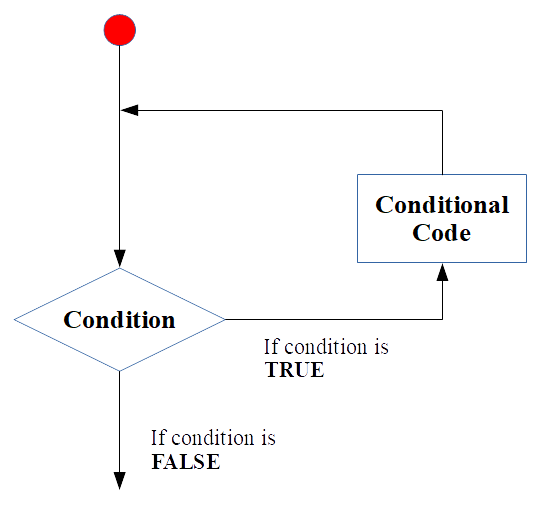
\includegraphics[width=0.4\linewidth]{skema_loop} 

}

\caption{Diagram umum loop (sumber: Primartha, 2018).}\label{fig:loop}
\end{figure}

\subsection{For Loop}\label{for-loop}

Mengulangi sebuah \emph{statement} atau sekelompok \emph{statement}
sebanyak nilai yang ditentukan di awal. Jadi operasi akan terus
dilakukan sampai dengan jumlah yang telah ditetapkan di awal atau dengan
kata lain tes kondisi (Jika jumlah pengulangan telah cukup) hanya akan
dilakukan di akhir. Secara sederhana bentuk dari \emph{for loop} dapat
dituliskan sebagai berikut:

\begin{Shaded}
\begin{Highlighting}[]
\ControlFlowTok{for}\NormalTok{ (value }\ControlFlowTok{in}\NormalTok{ vector)\{}
\NormalTok{  statements}
\NormalTok{\}}
\end{Highlighting}
\end{Shaded}

Berikut adalah contoh sintaks penerapan \emph{for loop}:

\begin{Shaded}
\begin{Highlighting}[]
\CommentTok{# Membuat vektor numerik}
\NormalTok{vektor <-}\StringTok{ }\KeywordTok{c}\NormalTok{(}\DecValTok{1}\OperatorTok{:}\DecValTok{5}\NormalTok{)}

\CommentTok{# loop }
\ControlFlowTok{for}\NormalTok{(i }\ControlFlowTok{in}\NormalTok{ vektor)\{}
  \KeywordTok{print}\NormalTok{(i)}
\NormalTok{\}}
\end{Highlighting}
\end{Shaded}

\begin{verbatim}
## [1] 1
## [1] 2
## [1] 3
## [1] 4
## [1] 5
\end{verbatim}

\emph{Loop} akan dimulai dari blok \emph{statement for} sampai dengan
\texttt{print(i)}. Berdasarkan \emph{loop} pada contoh tersebut,
\emph{loop} hanya dilakukan sebanyak 5 kali sesuai dengan jumlah vektor
yang ada.

\subsection{While Loop}\label{while-loop}

\emph{While loop} merupakan loop yang digunakan ketika kita telah
menetapkan \emph{stop condition} sebelumnya. Blok \emph{statement}/kode
yang sama akan terus dijalankan sampai \emph{stop condition} ini
tercapai. \emph{Stop condition} akan di cek sebelum melakukan proses
\emph{loop}. Berikut adalah pola dari \emph{while loop} dapat dituliskan
sebagai berikut:

\begin{Shaded}
\begin{Highlighting}[]
\ControlFlowTok{while}\NormalTok{ (test_expression)\{}
\NormalTok{  statement}
\NormalTok{\}}
\end{Highlighting}
\end{Shaded}

Berikut adalah contoh penerapan dari \emph{while loop}:

\begin{Shaded}
\begin{Highlighting}[]
\NormalTok{coba <-}\StringTok{ }\KeywordTok{c}\NormalTok{(}\StringTok{"Contoh"}\NormalTok{)}
\NormalTok{counter <-}\StringTok{ }\DecValTok{1}

\CommentTok{# loop}
\ControlFlowTok{while}\NormalTok{ (counter}\OperatorTok{<}\DecValTok{5}\NormalTok{)\{}
  \CommentTok{# print vektor}
  \KeywordTok{print}\NormalTok{(coba)}
  \CommentTok{# tambahkan nilai counter sehingga proses terus berlangsung sampai counter = 5 }
\NormalTok{  counter <-}\StringTok{ }\NormalTok{counter }\OperatorTok{+}\StringTok{ }\DecValTok{1}
\NormalTok{\}}
\end{Highlighting}
\end{Shaded}

\begin{verbatim}
## [1] "Contoh"
## [1] "Contoh"
## [1] "Contoh"
## [1] "Contoh"
\end{verbatim}

\emph{Loop} akan dimulai dari blok \emph{statement while} sampai dengan
\emph{counter} \textless{}- 1. \emph{Loop} hanya akan dilakukan
sepanjang nilai \emph{counter} \textless{} 5.

\subsection{Repeat Loop}\label{repeat-loop}

\emph{Repeat loop} akan menjalankan \emph{statement}/kode yang sama
berulang-ulang hingga \emph{stop condition} tercapai. Berikut adalah
pola dari \emph{repeat loop}.

\begin{Shaded}
\begin{Highlighting}[]
\ControlFlowTok{repeat}\NormalTok{ \{}
\NormalTok{  commands}
  \ControlFlowTok{if}\NormalTok{(condition)\{}
    \ControlFlowTok{break}
\NormalTok{  \}}
\NormalTok{\}}
\end{Highlighting}
\end{Shaded}

Berikut adalah contoh penerapan dari \emph{repeat loop}:

\begin{Shaded}
\begin{Highlighting}[]
\NormalTok{coba <-}\StringTok{ }\KeywordTok{c}\NormalTok{(}\StringTok{"contoh"}\NormalTok{)}
\NormalTok{counter <-}\StringTok{ }\DecValTok{1}
\ControlFlowTok{repeat}\NormalTok{ \{}
  \KeywordTok{print}\NormalTok{(coba)}
\NormalTok{  counter <-}\StringTok{ }\NormalTok{counter }\OperatorTok{+}\StringTok{ }\DecValTok{1}
  \ControlFlowTok{if}\NormalTok{(counter }\OperatorTok{<}\StringTok{ }\DecValTok{5}\NormalTok{)\{}
\ControlFlowTok{break}
\NormalTok{  \}}
\NormalTok{\}}
\end{Highlighting}
\end{Shaded}

\begin{verbatim}
## [1] "contoh"
\end{verbatim}

\emph{Loop} akan dimulai dari blok \emph{statement while} sampai dengan
\emph{break}. \emph{Loop} hanya akan dilakukan sepanjang nilai
\emph{counter} \textless{} 5. Hasil yang diperoleh berbeda dengan
\emph{while loop}, dimana kita memperoleh 4 buah kata ``contoh''. Hal
ini disebabkan karena \emph{repeat loop} melakukan pengecekan \emph{stop
condition} tidak di awal loop seperti \emph{while loop} sehingga
berapapun nilainya, selama nilainya sesuai dengan \emph{stop condition}
maka \emph{loop} akan dihentikan. Hal ini berbeda dengan \emph{while
loop} dimana proses dilakukan berulang-ulang sampai jumlahnya mendekati
\emph{stop condition}.

\subsection{Break}\label{break}

\emph{Break} sebenarnya bukan bagian dari \emph{loop}, namun sering
digunakan dalam \emph{loop}. \emph{Break} dapat digunakan pada
\emph{loop} manakala dirasa perlu, yaitu saat kondisi yang disyaratkan
pada \emph{break} tercapai.

Berikut adalah contoh penerapan \emph{break} pada beberapa jenis
\emph{loop}.

\begin{Shaded}
\begin{Highlighting}[]
\CommentTok{# for loop}
\NormalTok{a =}\StringTok{ }\KeywordTok{c}\NormalTok{(}\DecValTok{2}\NormalTok{,}\DecValTok{4}\NormalTok{,}\DecValTok{6}\NormalTok{,}\DecValTok{8}\NormalTok{,}\DecValTok{10}\NormalTok{,}\DecValTok{12}\NormalTok{,}\DecValTok{14}\NormalTok{)}
\ControlFlowTok{for}\NormalTok{(i }\ControlFlowTok{in}\NormalTok{ a)\{}
  \ControlFlowTok{if}\NormalTok{(i}\OperatorTok{>}\DecValTok{8}\NormalTok{)\{}
    \ControlFlowTok{break}
\NormalTok{  \}}
  \KeywordTok{print}\NormalTok{(i)}
\NormalTok{\}}
\end{Highlighting}
\end{Shaded}

\begin{verbatim}
## [1] 2
## [1] 4
## [1] 6
## [1] 8
\end{verbatim}

\begin{Shaded}
\begin{Highlighting}[]
\CommentTok{# while loop}
\NormalTok{a =}\StringTok{ }\DecValTok{2}
\NormalTok{b =}\StringTok{ }\DecValTok{4}
\ControlFlowTok{while}\NormalTok{(a}\OperatorTok{<}\DecValTok{7}\NormalTok{)\{}
  \KeywordTok{print}\NormalTok{(a)}
\NormalTok{  a =}\StringTok{ }\NormalTok{a }\OperatorTok{+}\DecValTok{1}
  \ControlFlowTok{if}\NormalTok{(b}\OperatorTok{+}\NormalTok{a}\OperatorTok{>}\DecValTok{10}\NormalTok{)\{}
    \ControlFlowTok{break}
\NormalTok{  \}}
\NormalTok{\}}
\end{Highlighting}
\end{Shaded}

\begin{verbatim}
## [1] 2
## [1] 3
## [1] 4
## [1] 5
## [1] 6
\end{verbatim}

\begin{Shaded}
\begin{Highlighting}[]
\CommentTok{# repeat loop}
\NormalTok{a =}\StringTok{ }\DecValTok{1}
\ControlFlowTok{repeat}\NormalTok{\{}
  \KeywordTok{print}\NormalTok{(a)}
\NormalTok{  a =}\StringTok{ }\NormalTok{a}\OperatorTok{+}\DecValTok{1}
  \ControlFlowTok{if}\NormalTok{(a}\OperatorTok{>}\DecValTok{6}\NormalTok{)\{}
    \ControlFlowTok{break}
\NormalTok{  \}}
\NormalTok{\}}
\end{Highlighting}
\end{Shaded}

\begin{verbatim}
## [1] 1
## [1] 2
## [1] 3
## [1] 4
## [1] 5
## [1] 6
\end{verbatim}

\section{Decision Making}\label{decision-making}

\emph{Decicion Making} atau sering disebut sebagai \emph{if then else
statement} merupakan bentuk percabagan yang digunakan manakala kita
ingin agar program dapat melakukan pengujian terhadap syarat kondisi
tertentu. Pada Table 5 disajikan daftar percabangan yang digunakan pada
\texttt{R}.

\textbf{Table 5} Daftar percabangan pada \texttt{R}

\begin{longtable}[]{@{}ll@{}}
\toprule
\begin{minipage}[b]{0.15\columnwidth}\raggedright\strut
\textbf{Statement}\strut
\end{minipage} & \begin{minipage}[b]{0.79\columnwidth}\raggedright\strut
\textbf{Keterangan}\strut
\end{minipage}\tabularnewline
\midrule
\endhead
\begin{minipage}[t]{0.15\columnwidth}\raggedright\strut
\emph{if statement}\strut
\end{minipage} & \begin{minipage}[t]{0.79\columnwidth}\raggedright\strut
\emph{if statement} hanya terdiri atas sebuah ekspresi \emph{Boolean},
dan diikuti satu atau lebih \emph{statement}\strut
\end{minipage}\tabularnewline
\begin{minipage}[t]{0.15\columnwidth}\raggedright\strut
\emph{if\ldots{}else statement}\strut
\end{minipage} & \begin{minipage}[t]{0.79\columnwidth}\raggedright\strut
\emph{if else statement} terdiri atas beberapa buah ekspresi
\emph{Boolean}. Ekspressi \emph{Boolean} berikutnya akan dijalankan jika
ekspresi *Boolan sebelumnya bernilai FALSE\strut
\end{minipage}\tabularnewline
\begin{minipage}[t]{0.15\columnwidth}\raggedright\strut
\emph{switch statement}\strut
\end{minipage} & \begin{minipage}[t]{0.79\columnwidth}\raggedright\strut
\emph{switch statement} digunakan untuk mengevaluasi sebuah variabel
beberapa pilihan\strut
\end{minipage}\tabularnewline
\bottomrule
\end{longtable}

\subsection{if statement}\label{if-statement}

Pola \emph{if statement} disajikan pada Figure \ref{fig:ifstatement}

\begin{figure}

{\centering 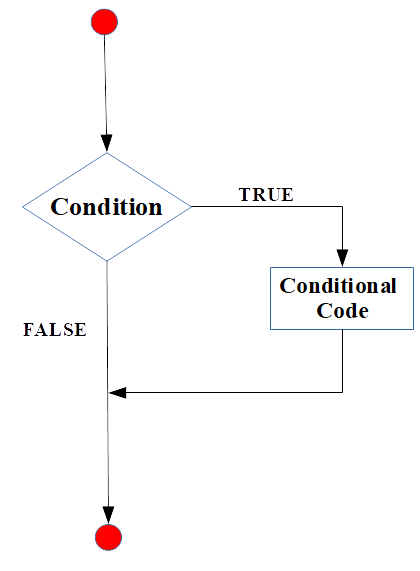
\includegraphics[width=0.4\linewidth]{ifstatement} 

}

\caption{Diagram if statement (sumber: Primartha, 2018).}\label{fig:ifstatement}
\end{figure}

Berikut adalah contoh penerapan \emph{if statement}:

\begin{Shaded}
\begin{Highlighting}[]
\NormalTok{x <-}\StringTok{ }\KeywordTok{c}\NormalTok{(}\DecValTok{1}\OperatorTok{:}\DecValTok{5}\NormalTok{)}
\ControlFlowTok{if}\NormalTok{(}\KeywordTok{is.vector}\NormalTok{(x))\{}
  \KeywordTok{print}\NormalTok{(}\StringTok{"x adalah sebuah vector"}\NormalTok{)}
\NormalTok{\}}
\end{Highlighting}
\end{Shaded}

\begin{verbatim}
## [1] "x adalah sebuah vector"
\end{verbatim}

\subsection{if else statement}\label{if-else-statement}

Pola dari \emph{if else statement} disajikan pada Figure
\ref{fig:ifelse}

\begin{figure}

{\centering 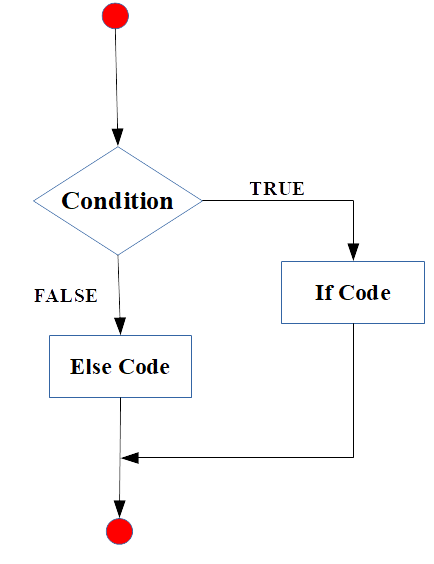
\includegraphics[width=0.4\linewidth]{ifelse} 

}

\caption{Diagram if else statement (sumber: Primartha, 2018).}\label{fig:ifelse}
\end{figure}

Berikut adalah contoh penerapan \emph{if else statement}:

\begin{Shaded}
\begin{Highlighting}[]
\NormalTok{x <-}\StringTok{ }\KeywordTok{c}\NormalTok{(}\StringTok{"Andi"}\NormalTok{,}\StringTok{"Iwan"}\NormalTok{, }\StringTok{"Adi"}\NormalTok{)}
\ControlFlowTok{if}\NormalTok{(}\StringTok{"Rina"} \OperatorTok\StringTok{ }\NormalTok{x)\{}
  \KeywordTok{print}\NormalTok{(}\StringTok{"Rina ditemukan"}\NormalTok{)}
\NormalTok{\} }\ControlFlowTok{else} \ControlFlowTok{if}\NormalTok{(}\StringTok{"Adi"} \OperatorTok\StringTok{ }\NormalTok{x)\{}
  \KeywordTok{print}\NormalTok{(}\StringTok{"Adi ditemukan"}\NormalTok{)}
\NormalTok{\} }\ControlFlowTok{else}\NormalTok{\{}
  \KeywordTok{print}\NormalTok{(}\StringTok{"tidak ada yang ditemukan"}\NormalTok{)}
\NormalTok{\}}
\end{Highlighting}
\end{Shaded}

\begin{verbatim}
## [1] "Adi ditemukan"
\end{verbatim}

\subsection{switch statement}\label{switch-statement}

Pola dari \emph{switch statement} disajikan pada Figure \ref{fig:switch}

\begin{figure}

{\centering 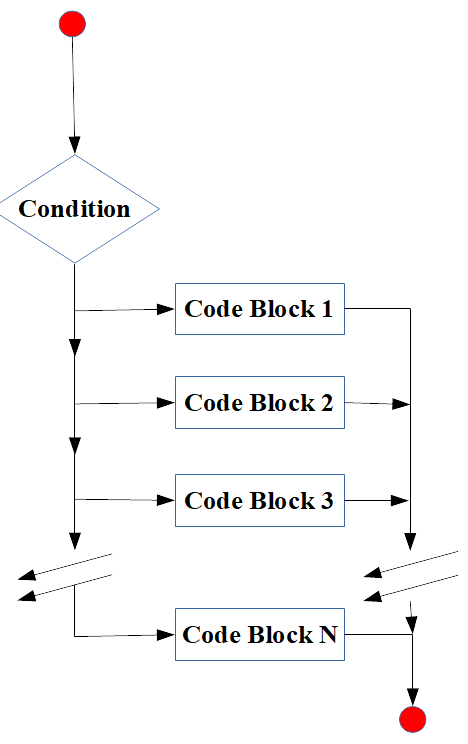
\includegraphics[width=0.4\linewidth]{switch} 

}

\caption{Diagram switch statement (sumber: Primartha, 2018).}\label{fig:switch}
\end{figure}

Berikut adalah contoh penerapan \emph{switch statement}:

\begin{Shaded}
\begin{Highlighting}[]
\NormalTok{y =}\StringTok{ }\DecValTok{3}

\NormalTok{x =}\StringTok{ }\ControlFlowTok{switch}\NormalTok{(}
\NormalTok{  y,}
  \StringTok{"Selamat Pagi"}\NormalTok{,}
  \StringTok{"Selamat Siang"}\NormalTok{,}
  \StringTok{"Selamat Sore"}\NormalTok{,}
  \StringTok{"Selamat Malam"}
\NormalTok{)}

\KeywordTok{print}\NormalTok{(x)}
\end{Highlighting}
\end{Shaded}

\begin{verbatim}
## [1] "Selamat Sore"
\end{verbatim}

\section{Fungsi}\label{fungsi}

Fungsi merupakan sekumpulan instruksi atau \emph{statement} yang dapat
melakukan tugas khusus. Sebagai contoh fungsi perkalian untuk
menyelesaikan operasi perkalian, fungsi pemangkatan hanya untuk operasi
pemangkatan, dll.

Pada \texttt{R} terdapat 2 jenis fungsi, yaitu: \emph{build in fuction}
dan \emph{user define function}. \emph{build in fnction} merupakan
fungsi bawaan \texttt{R} saat pertama kita menginstall \texttt{R}.
Contohnya adalah \texttt{mean()}, \texttt{sum()}, \texttt{ls()},
\texttt{rm()}, dll. Sedangkan \emph{user define fuction} merupakan
fungsi-fungsi yang dibuat sendiri oleh pengguna.

Fungsi-fungsi buatan pengguna haruslah dideklarasikan (dibuat) terlebih
dahulu sebelum dapat dijalankan. Pola pembentukan fungsi adalah sebagai
berikut:

\begin{Shaded}
\begin{Highlighting}[]
\NormalTok{function_name <-}\StringTok{ }\ControlFlowTok{function}\NormalTok{(argument_}\DecValTok{1}\NormalTok{, argument_}\DecValTok{2}\NormalTok{, ...)\{}
  \ControlFlowTok{function}\NormalTok{ body}
\NormalTok{\}}
\end{Highlighting}
\end{Shaded}

\begin{quote}
\textbf{Note: }

\begin{itemize}
\tightlist
\item
  \textbf{function\_name} : Nama dari fungsi \texttt{R}. \texttt{R} akan
  menyimpan fungsi tersebut sebagai objek
\item
  \textbf{argument\_1, argument\_2,\ldots{}} : \emph{Argument} bersifat
  opsional (tidak wajib). \emph{Argument} dapat digunakan untuk memberi
  inputan kepada fungsi
\item
  \textbf{function body} : Merupakan inti dari fungsi. Fuction body
  dapat terdiri atas 0 statement (kosong) hingga banyak statement.
\item
  \textbf{return} : Fungsi ada yang memiliki \emph{output} atau
  \emph{return value} ada juga yang tidak. Jika fungsi memiliki
  \emph{return value} maka \emph{return value} dapat diproses lebih
  lanjut
\end{itemize}
\end{quote}

Berikut adalah contoh penerapan \emph{user define function}:

\begin{Shaded}
\begin{Highlighting}[]
\CommentTok{# Fungsi tanpa argument}
\NormalTok{bilang <-}\StringTok{ }\ControlFlowTok{function}\NormalTok{()\{}
  \KeywordTok{print}\NormalTok{(}\StringTok{"Hello World!!"}\NormalTok{)}
\NormalTok{\}}

\CommentTok{# Print}
\KeywordTok{bilang}\NormalTok{()}
\end{Highlighting}
\end{Shaded}

\begin{verbatim}
## [1] "Hello World!!"
\end{verbatim}

\begin{Shaded}
\begin{Highlighting}[]
\CommentTok{# Fungsi dengan argumen}
\NormalTok{tambah <-}\StringTok{ }\ControlFlowTok{function}\NormalTok{(a,b)\{}
  \KeywordTok{print}\NormalTok{(a}\OperatorTok{+}\NormalTok{b)}
\NormalTok{\}}

\CommentTok{# Print}
\KeywordTok{tambah}\NormalTok{(}\DecValTok{5}\NormalTok{,}\DecValTok{3}\NormalTok{)}
\end{Highlighting}
\end{Shaded}

\begin{verbatim}
## [1] 8
\end{verbatim}

\begin{Shaded}
\begin{Highlighting}[]
\CommentTok{# Fungsi dengan return value}
\NormalTok{kali <-}\StringTok{ }\ControlFlowTok{function}\NormalTok{(a,b)\{}
  \KeywordTok{return}\NormalTok{(a}\OperatorTok{*}\NormalTok{b)}
\NormalTok{\}}

\CommentTok{# Print}
\KeywordTok{kali}\NormalTok{(}\DecValTok{4}\NormalTok{,}\DecValTok{3}\NormalTok{)}
\end{Highlighting}
\end{Shaded}

\begin{verbatim}
## [1] 12
\end{verbatim}

\section{Referensi}\label{referensi-1}

\begin{enumerate}
\def\labelenumi{\arabic{enumi}.}
\tightlist
\item
  Primartha, R. 2018. \textbf{Belajar Machine Learning Teori dan
  Praktik}. Penerbit Informatika : Bandung.
\item
  Rosadi,D. 2016. \textbf{Analisis Statistika dengan R}. Gadjah Mada
  University Press: Yogyakarta.
\item
  STHDA. \textbf{Easy R Programming Basics}.
  \url{http://www.sthda.com/english/wiki/easy-r-programming-basics}
\item
  Venables, W.N. Smith D.M. and R Core Team. 2018. \textbf{An
  Introduction to R}. R Manuals.
\item
  The R Core Team. 2018. \textbf{R: A Language and Environment for
  Statistical Computing}. R Manuals.
\end{enumerate}

\chapter{Methods}\label{methods}

We describe our methods in this chapter.

\chapter{Applications}\label{applications}

Some \emph{significant} applications are demonstrated in this chapter.

\section{Example one}\label{example-one}

\section{Example two}\label{example-two}

\chapter{Final Words}\label{final-words}

We have finished a nice book.

\bibliography{book.bib,packages.bib}


\end{document}
